\chapter{Results}

A set of twenty ligands from the PDBbind-CN database has been downloaded and used for testing
purposes (common core construction as well as mutation routes). It
should be noted, however, that the common core of pairs of these ligands
in some cases violate the rules of Transformato concerning a valid
maximum common substructure, i.e. dummy regions are connected by more
than one atom to the common core (which basically implies that the
atom is part of a ring structure). 

In the current implementation of the mutation algorithm this problem
is solved by a helper function which chooses one of the possible connections
between one of the atoms to the common core. For the following processing
of the mutation algorithm, this connection is arbitrarily distinguished
and the other ones removed. 


\section{Visualizations}

The mutation route can be visualized using a color gradient (additionally
to numbering, see figures above).

Py3dMol is used for a 3D-animation of the mutation process. Fig. 5.1
shows two molecules and their shared common core.

\begin{figure}
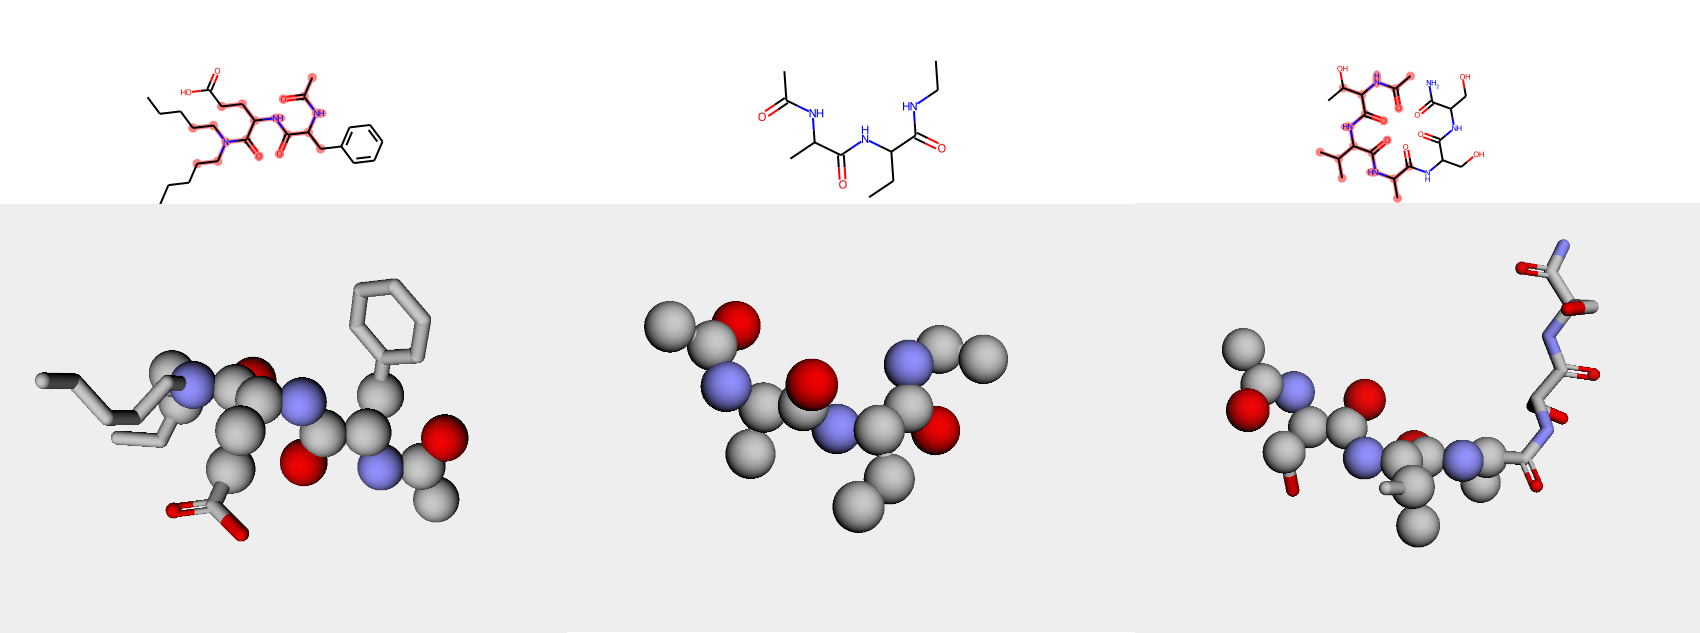
\includegraphics[scale=0.35]{trafo_py3d_1verkleinert}

\caption{Visualization of the mutation route using Py3dmol; upper row: Rdkit-representations
of both molecules and the common core; lower row: Py3Dmol visualizations;
left and right: molecules; middle: common core of both molecules}

\end{figure}


\section{Scoring schemes}

Several scoring schemes have been implemented to assess and compare
the mutation routes proposed by the new algorithms.\\
1) Betweenness centrality: Betweenness centrality measures the number
of shortest paths going through a specific node\cite{Newman.2010}. More central atoms
will have a higher centrality coefficient, whereas atoms remote from
the common core will have a lower (e.g., the last atom of a chain
has a coefficient of 0 because no path between two other atoms visits
the representing node). After each step, the node is removed from
the graph.
For avoiding undesired mutations, the maximum betweenness centrality
of all mutation steps is more decisive; hence the average of the mean
as well as the maximum betweenness centrality of all removed nodes
is shown below.

\begin{figure}[H]
	
	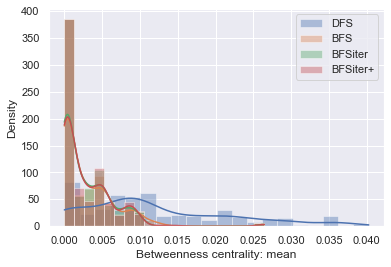
\includegraphics[scale=0.8]{betweenness_mean_all}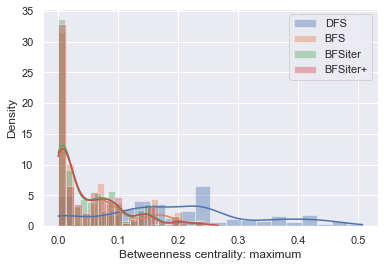
\includegraphics[scale=0.8]{betweenness_max_all}\caption{Betweenness centrality}
	
\end{figure}

2) Closeness centrality: Closeness centrality of a specific node is
given by the inverted distances between this node and all other nodes
of the graph\cite{Newman.2010}. Atoms more distant from the common core have a lower
closeness centrality.
For using this centrality measure as scoring function for the mutation
algorithms, the dummy region with the greatest number of atoms (simply
because this is probably the most \textquoteleft interesting\textquoteright{}
one, it would also be possible to take the average of all dummy regions
etc.) is selected. The closeness centrality of each removed node for
the full graph (i.e. all atoms, including already removed ones) is
computed. A 'good' mutation route should show an increase in closeness
centrality because at the beginning the atoms with a high distance
from the other atoms (and hence the common core atoms) are removed.
To evaluate this relation, linear regression of the computed centrality
values is performed. A higher slope indicates a 'better' mutation
route. Furthermore, correlation coefficients (Spearman, Kendall's
Tau) have been computed. Again, a higher correlation shows that the
closeness centrality of the atoms removed is increasing. Correlation
coefficients as well as regression coefficients are reported in the
tables below.

\begin{figure}[H]
	
	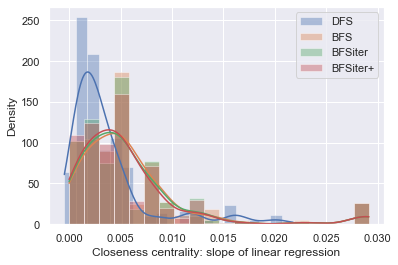
\includegraphics{closeness_slope_all}
	
	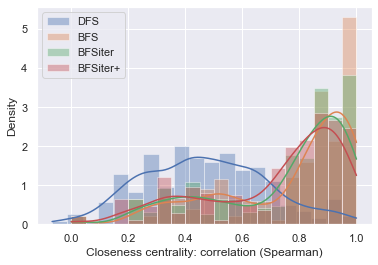
\includegraphics{closeness_spearman}
	
	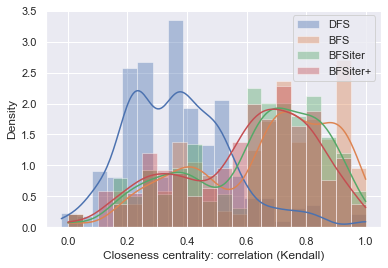
\includegraphics{closeness_kendall}\caption{Closeness centrality}
	
\end{figure}


3) ring-related scores: As stated above, the processing of ring structures
is of crucial importance and pronounced differences between DFS and
BFS occur. Four properties were calculated: The mean asymmetry at
ring opening was measured: After the first atom of a ring structure
is removed, usually two chains emerge. The length difference (i.e.
the difference in atom number) of these two chains was measured. If
both chains are equally long, the asymmetry is 0. 

The 'asymmetry during ring disassemby'-score does not only evaluate
the first atom removed from a ring, but checks at each mutation step
involving a ring atom if asymmetric chains emerge.

The 'mean number of open rings' indicates how many ring structures
are opened on average and the 'mean processing time of rings' determines
how many mutation steps it takes to completely process a ring (until
only one atom of the former ring structure is present).

It should be noted that even using the new algorithms it is possible
that a \textquoteleft broken\textquoteright{} ring stays for a while
in the system because atoms from other areas of the dummy region (e.g.,
a longer chain) are processed meanwhile. However, in contrast to DFS,
it should not happen that a ring near to the common core is opened
initially and hence the mean and maximum time should be significantly
shorter. 

In general, calculation of the scoring functions for the selection of ligands from the PDBbind data set (statistics are presented in table 1) match the expectations. 


\begin{table}
	
	\begin{tabular}{|>{\centering}p{2.5cm}|>{\centering}p{2.5cm}|>{\centering}p{2.5cm}|>{\centering}p{2.5cm}|>{\centering}p{2.5cm}|}
		\hline 
		number of processed routes & dummy atoms (mean) & atoms/dummy region (mean) & number of cycles (mean) & polycyclic {[}\%{]}\tabularnewline
		\hline 
		378 & 26.97 & 16.30 & 1.66 & 30.16\tabularnewline
		\hline 
	
	\end{tabular}\caption{statistics of PDBbind selection; number of processed routes: total number of computed routes for a specific combination of two molecules; dummy atoms (mean): average number of total dummy atoms in the computed mutation routes; atoms/dummy region (mean): number of total dummy atoms divided by the number of dummy regions; number of cycles (mean): average number of cycles in all mutation routes; polycyclic: percentage of mutation routes which involve polycyclic structures, i.e. there are atoms present that participate in multiple cycles }
\end{table}




\begin{figure}
	
	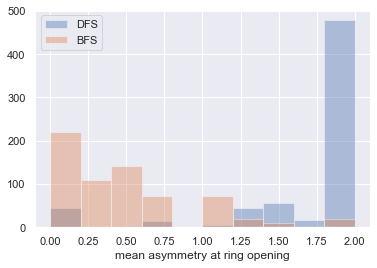
\includegraphics[scale=0.8]{mean_ass_beginn_bfs}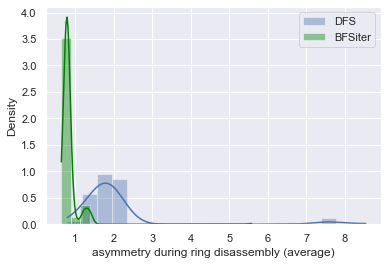
\includegraphics[scale=0.8]{mean_ass_total_onlyiter}
	
	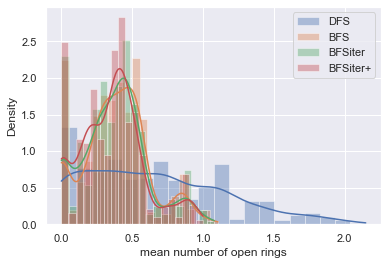
\includegraphics[scale=0.8]{mean_open_rings_all}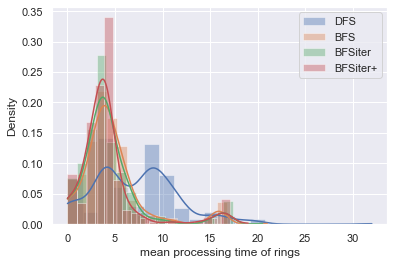
\includegraphics[scale=0.8]{mean_processing_all}
	
	\caption{Ring-related scores}
	
\end{figure}

In the plots presenting the scoring-functions, all molecule combinations
from the PDBbind data set are used. It could be insightful to use
only a subset (e.g. only molecules with dummy regions involving multiple
ring structures ore a minimum number of dummy atoms) or to try even a larger selection from the PDBbind database.

\section{Results for selected molecule pairs}

For selected pairs of small molecules, the relative solvation free energy differences have been determined using Transformato. 
An overview of the molecules and the corresponding mutation routes can be found in the appendix.

 {\color{red} (Vergleiche conclusion: Bis jetzt gab es 3 Versuche! Der erste mit größeren Molekuelen scheiterte - vielleicht auch, weil hier aufgrund der Wasserstoffproblematik teils falsche common cores berechnet wurden, vielleicht aber auch, weil die Molekuele einfach zu groß waren. Der zweite Versuch wurde fuer die 5 Molekuele in fig 5.5 angestellt, die Resultate sind aber nicht ganz vertrauenswuerdig. 3 Ergebnisse können nicht passen, da ein falscher common core verwundert wurde, weil die Wasserstoffe noch nicht richtig prozessiert wurden, also noch nicht vor common core-Generation und Mutationsfindung entfernt wurden (siehe 'processing of hydrogen atoms')! In einem 3. Versuch wurden zwei der Molekuele, naemlich Toluen und 2-Naphthol nochmals berechet, auch hier ist aber nicht ganz klar, ob alles passt...)}
 
Two such example pairs are toluene$\rightarrow$methanol and 2-naphthol$\rightarrow$methanol. In both cases, the corresponding common cores solely consist of one heavy atom, carbon or oxygen, respectively.

Calculation of the free energy difference indicates that for toluene$ 	\rightarrow $methanol the differences between the algorithms are negligible, but for 2-naphthol$ 	\rightarrow $methanol they are at least more pronounced (fig. 5.5 and table 5.2). 
Overlap plots for these mutations can be found in fig. 5.7,8 and 10. showing the differences between old and new mutation algorithms. Fig 5.9 also shows the evolution of the free energy estimate across the lambda states for 2-naphthol (vacuum and waterbox for old and new mutation algorithm).

The overlap plots for Naphthol$\rightarrow$Methanol exhibit a different pattern depending on the mutation route, but only for the simulation in vacuum, not for the waterbox, whereas for Toluene-Methanol hardly any difference is visible. (There are two adjacent states in the middle of the heavy atom transformation for naphthol/waterbox with a comparatively high overlap. Correspondingly, the plotting of the lambda states shows to steps in the middle of the simulation with almost no free energy change.)

Since the mutation route is fundamentally different depending on the algorithm (see fig. 7.2; the old algorithm starts next to the atom of the phenyl group that is connected to the methyl substituent - which serves as common core - and processes the rest of the atoms in a chain-like manner, whereas the new one starts at the atom with maximum distance from the substituent and proceeds in a symmetric way until the common core is attained), the result for toluene is highly astonishing. For the double ring structure of 2-naphthol stronger deviations occur; thus it would be insightful to determine which structural properties are of importance. 



\begin{table}
	
	\begin{tabular}{|>{\centering}p{5.5cm}|>{\centering}p{3.5cm}|>{\centering}p{3.5cm}|}
		\hline 
		mutation partners & old algorithm (DFS) & new algorithm (BFS) \tabularnewline
		\hline 
		toluene/methanol & -4.97 $ \pm $ 0.05 & -4.73 $ \pm $ 0.06 \tabularnewline
		\hline 
		2-naphthol/methanol & 1.04 $ \pm $ 0.05 & 0.85 $ \pm $ 0.22 \tabularnewline
		\hline 	
		
	\end{tabular}\caption{results for the mutation pairs methanol and toluene / naphthol }
\end{table}



\begin{figure}[H]
	
	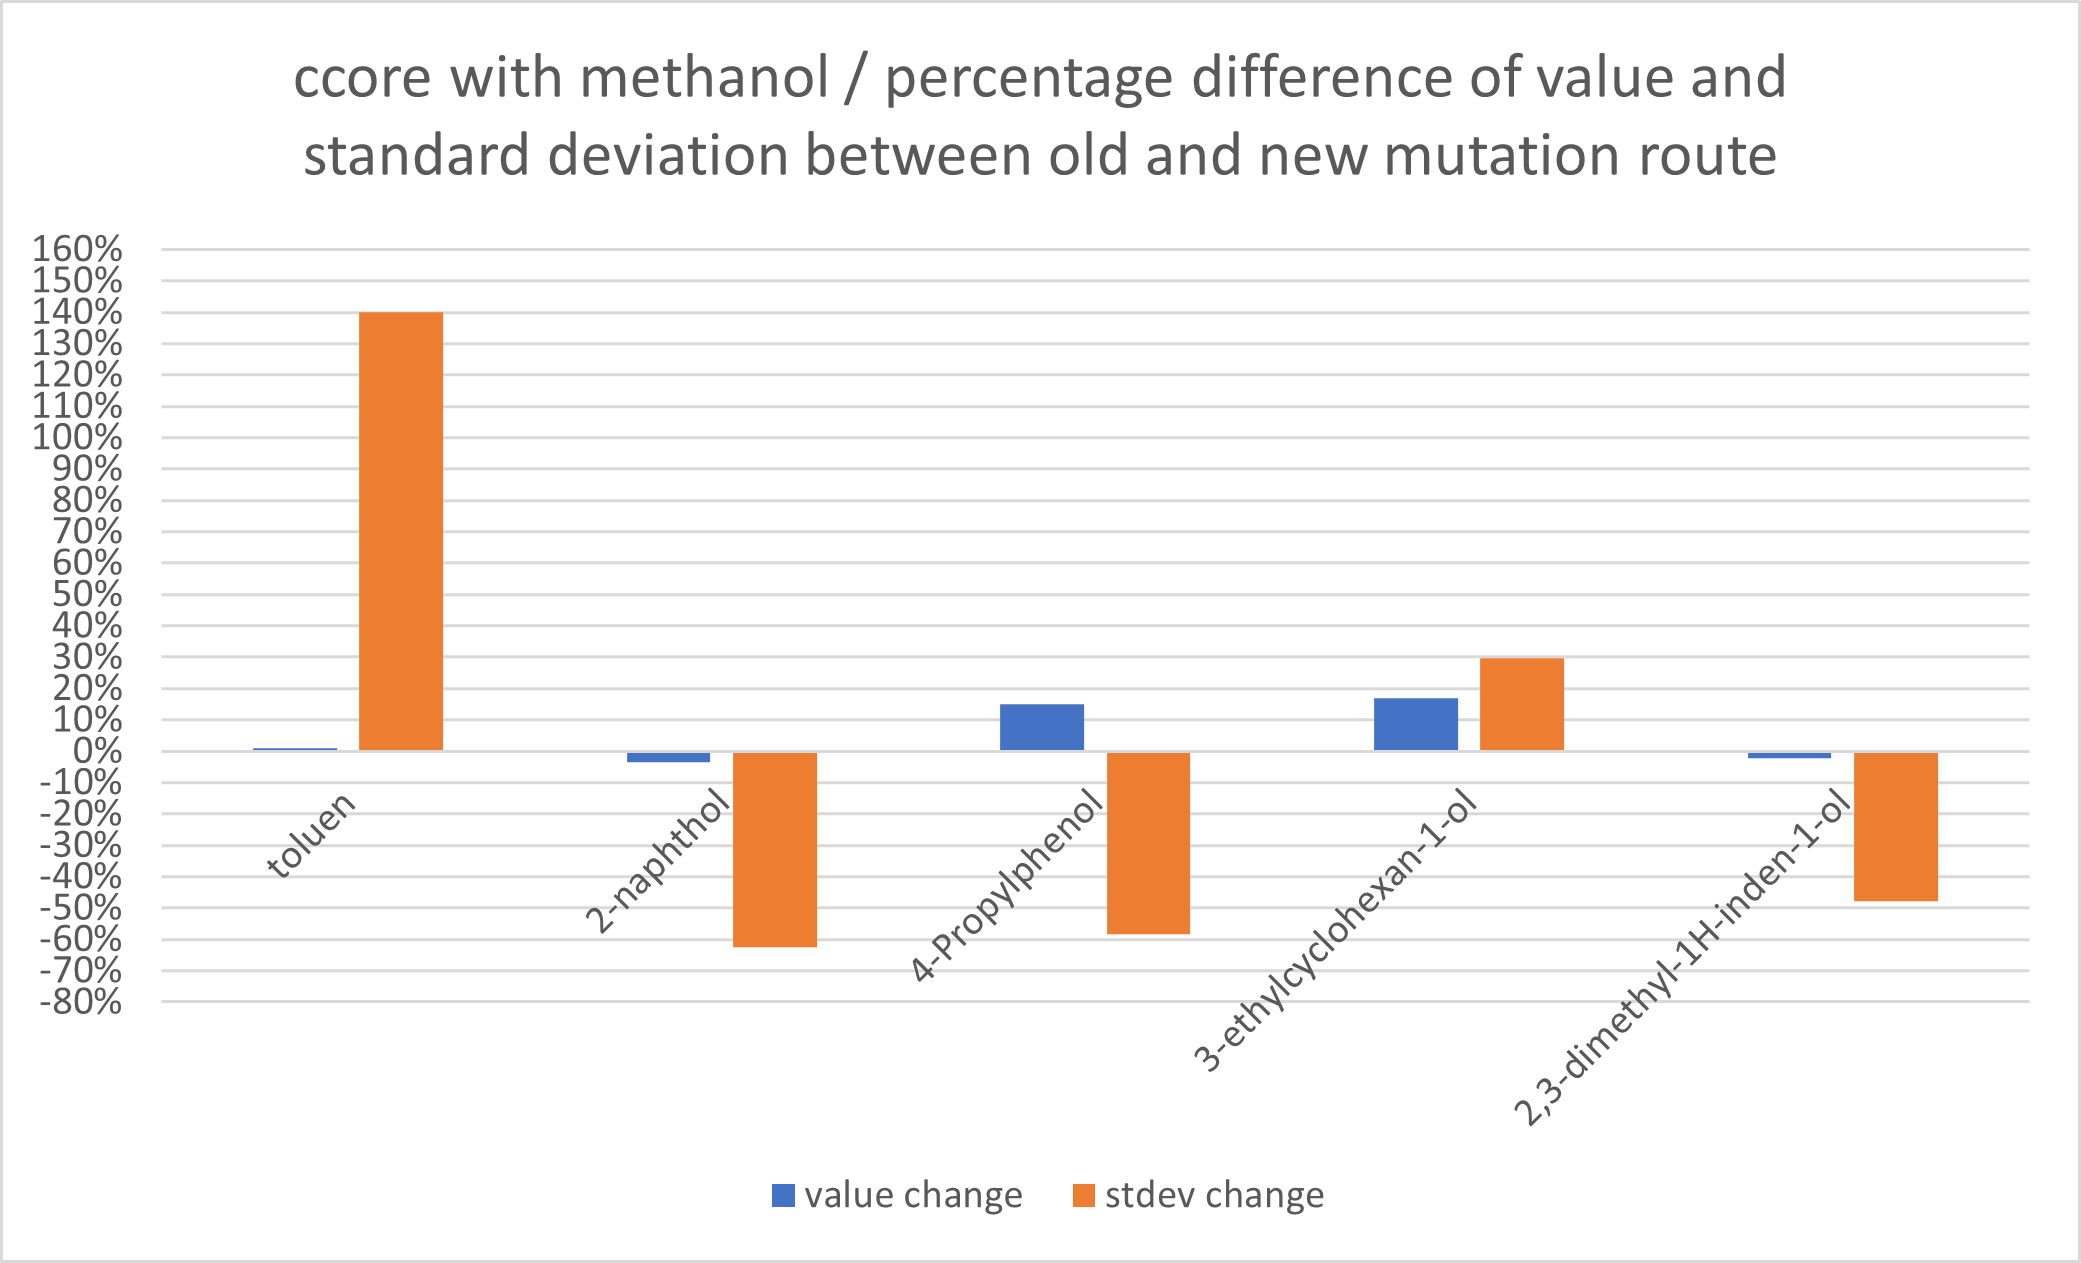
\includegraphics[scale=0.8]{molecules_v1_failed_barchart}
		
	
	{differences between old and new algorithm for selected molecules / 1. VERSUCH, DIESE RESULTATE SIND VERMUTLICH FEHLERHAFT; AUF JEDEN FALL IST BEI PROPYLPHENOL, ETHYLCYCLOHEXAN und DIMETHYLINDENOL DER FALSCHE CCORE VERWENDET WORDEN (aufgrund nicht entfernter Wasserstoffatome!)}
	
	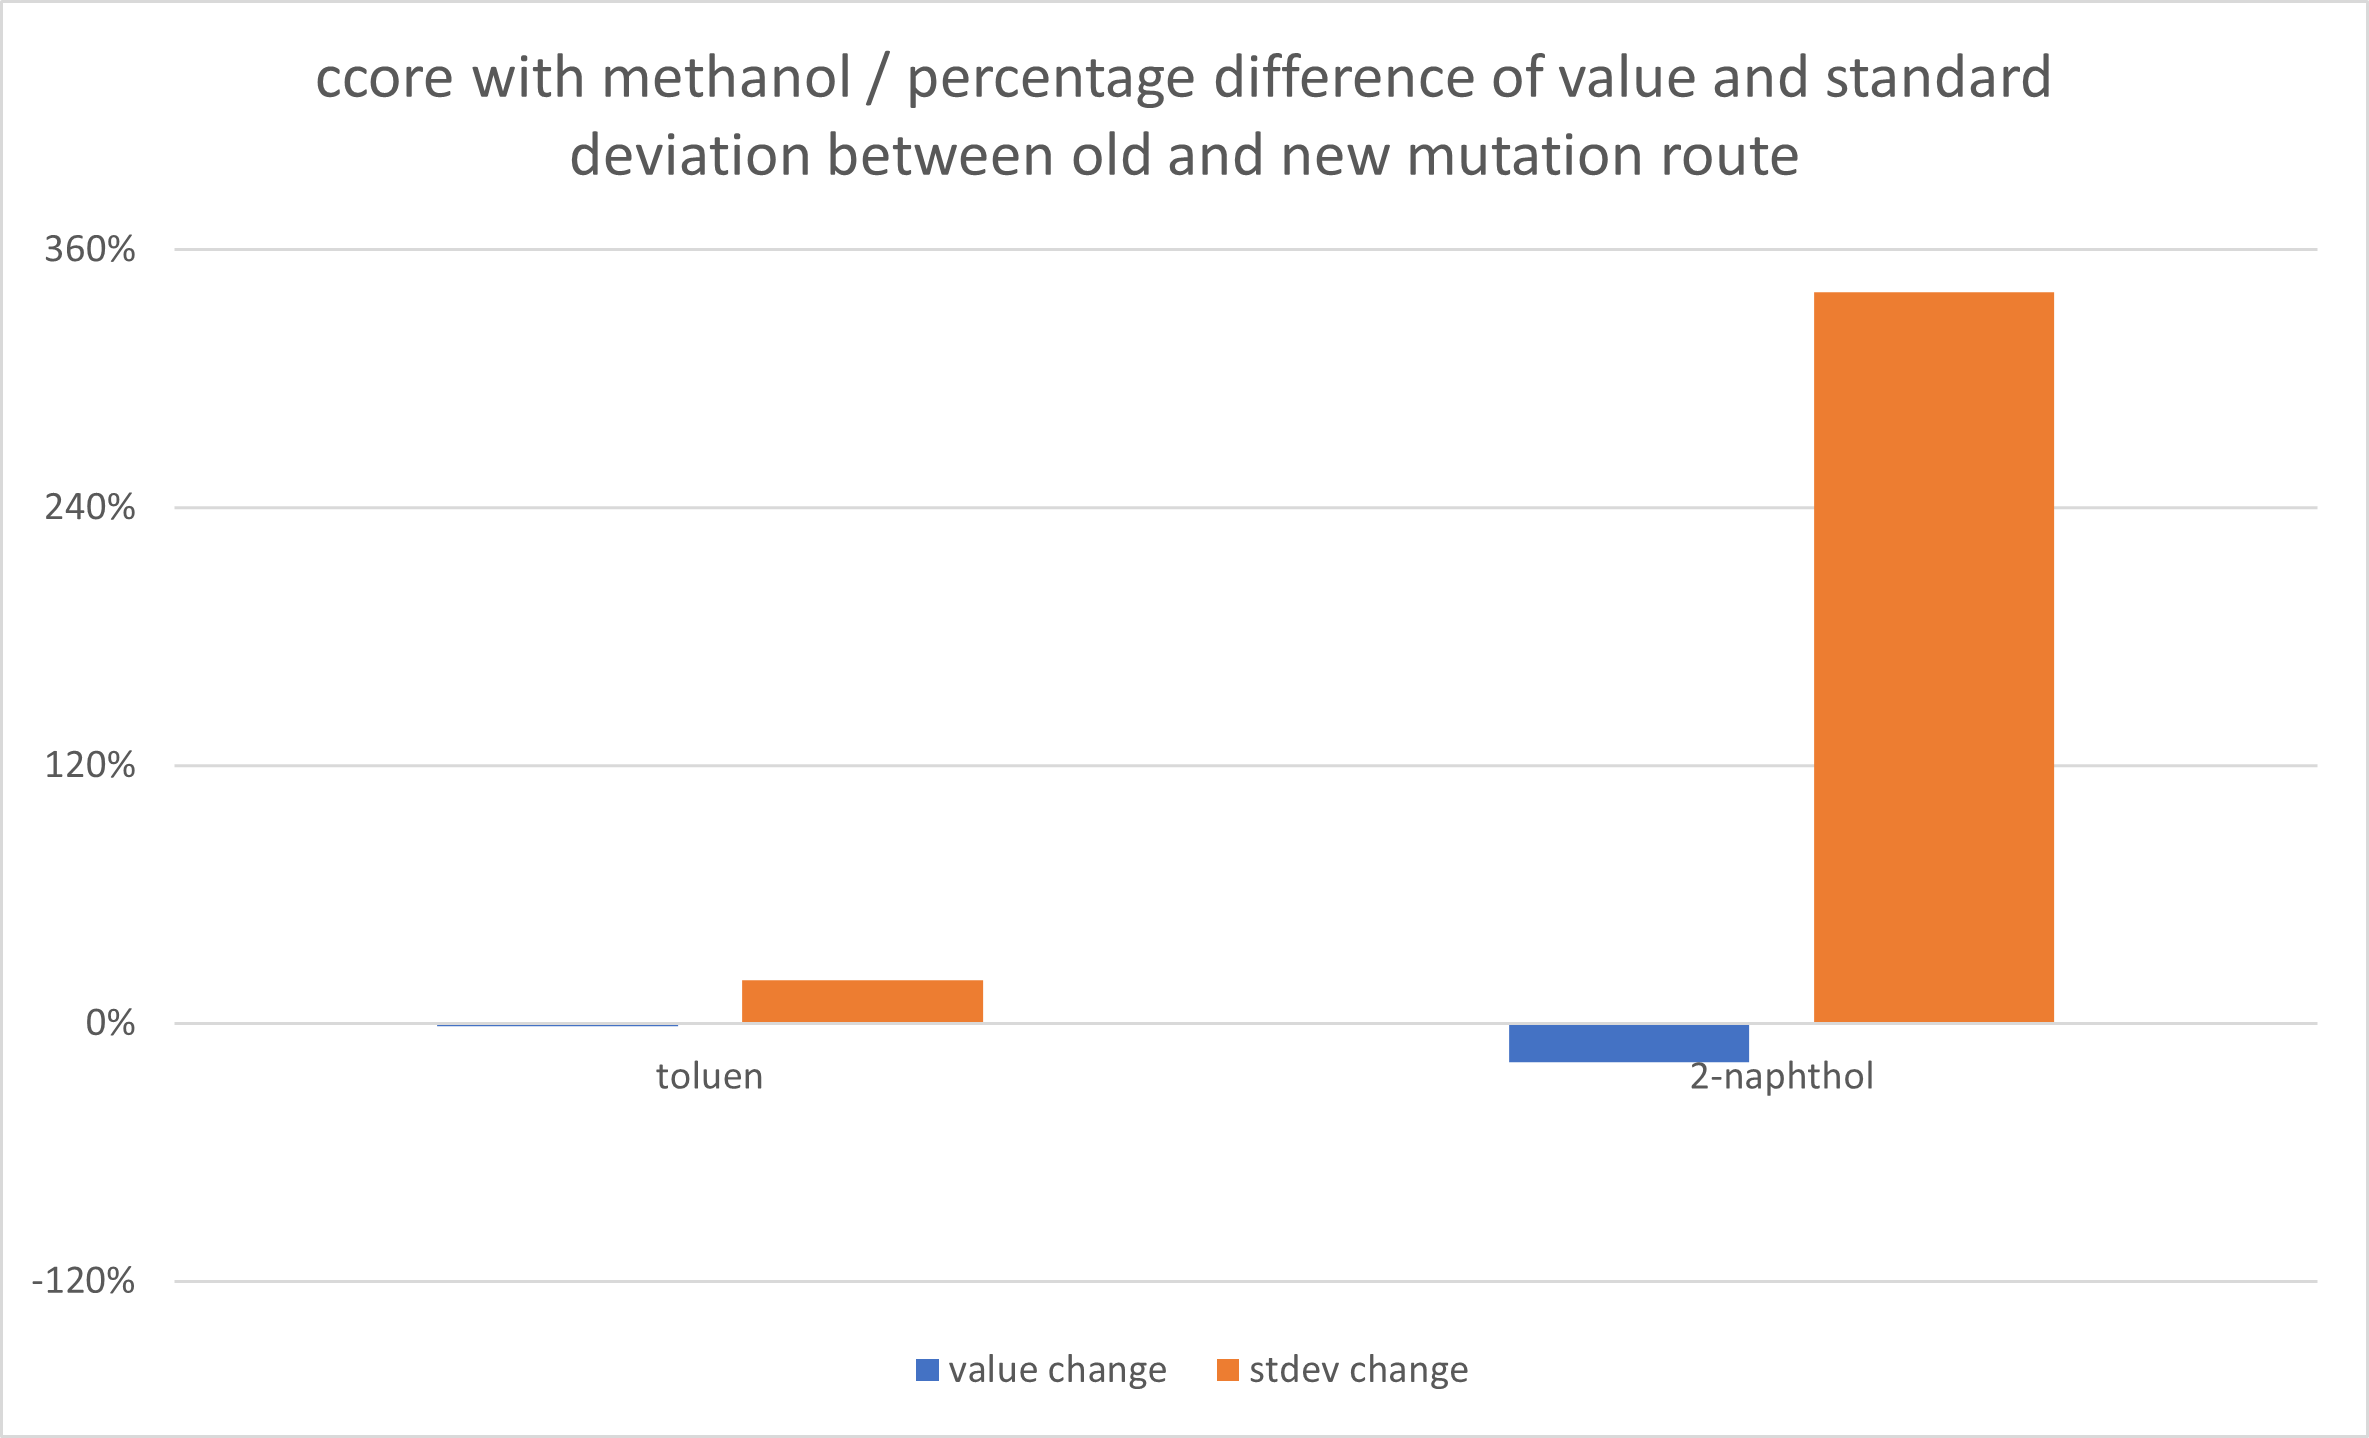
\includegraphics[scale=0.8]{2molecules_v2_barchart}
	
	
	\caption{differences between old and new algorithm for selected molecules / 2. VERSUCH, muss ebenfalls nochmals ueberprueft werden}
	
\end{figure}


\begin{figure}[h] 
	\centering
	\subfigure[naphthol/vacuum old]{%
		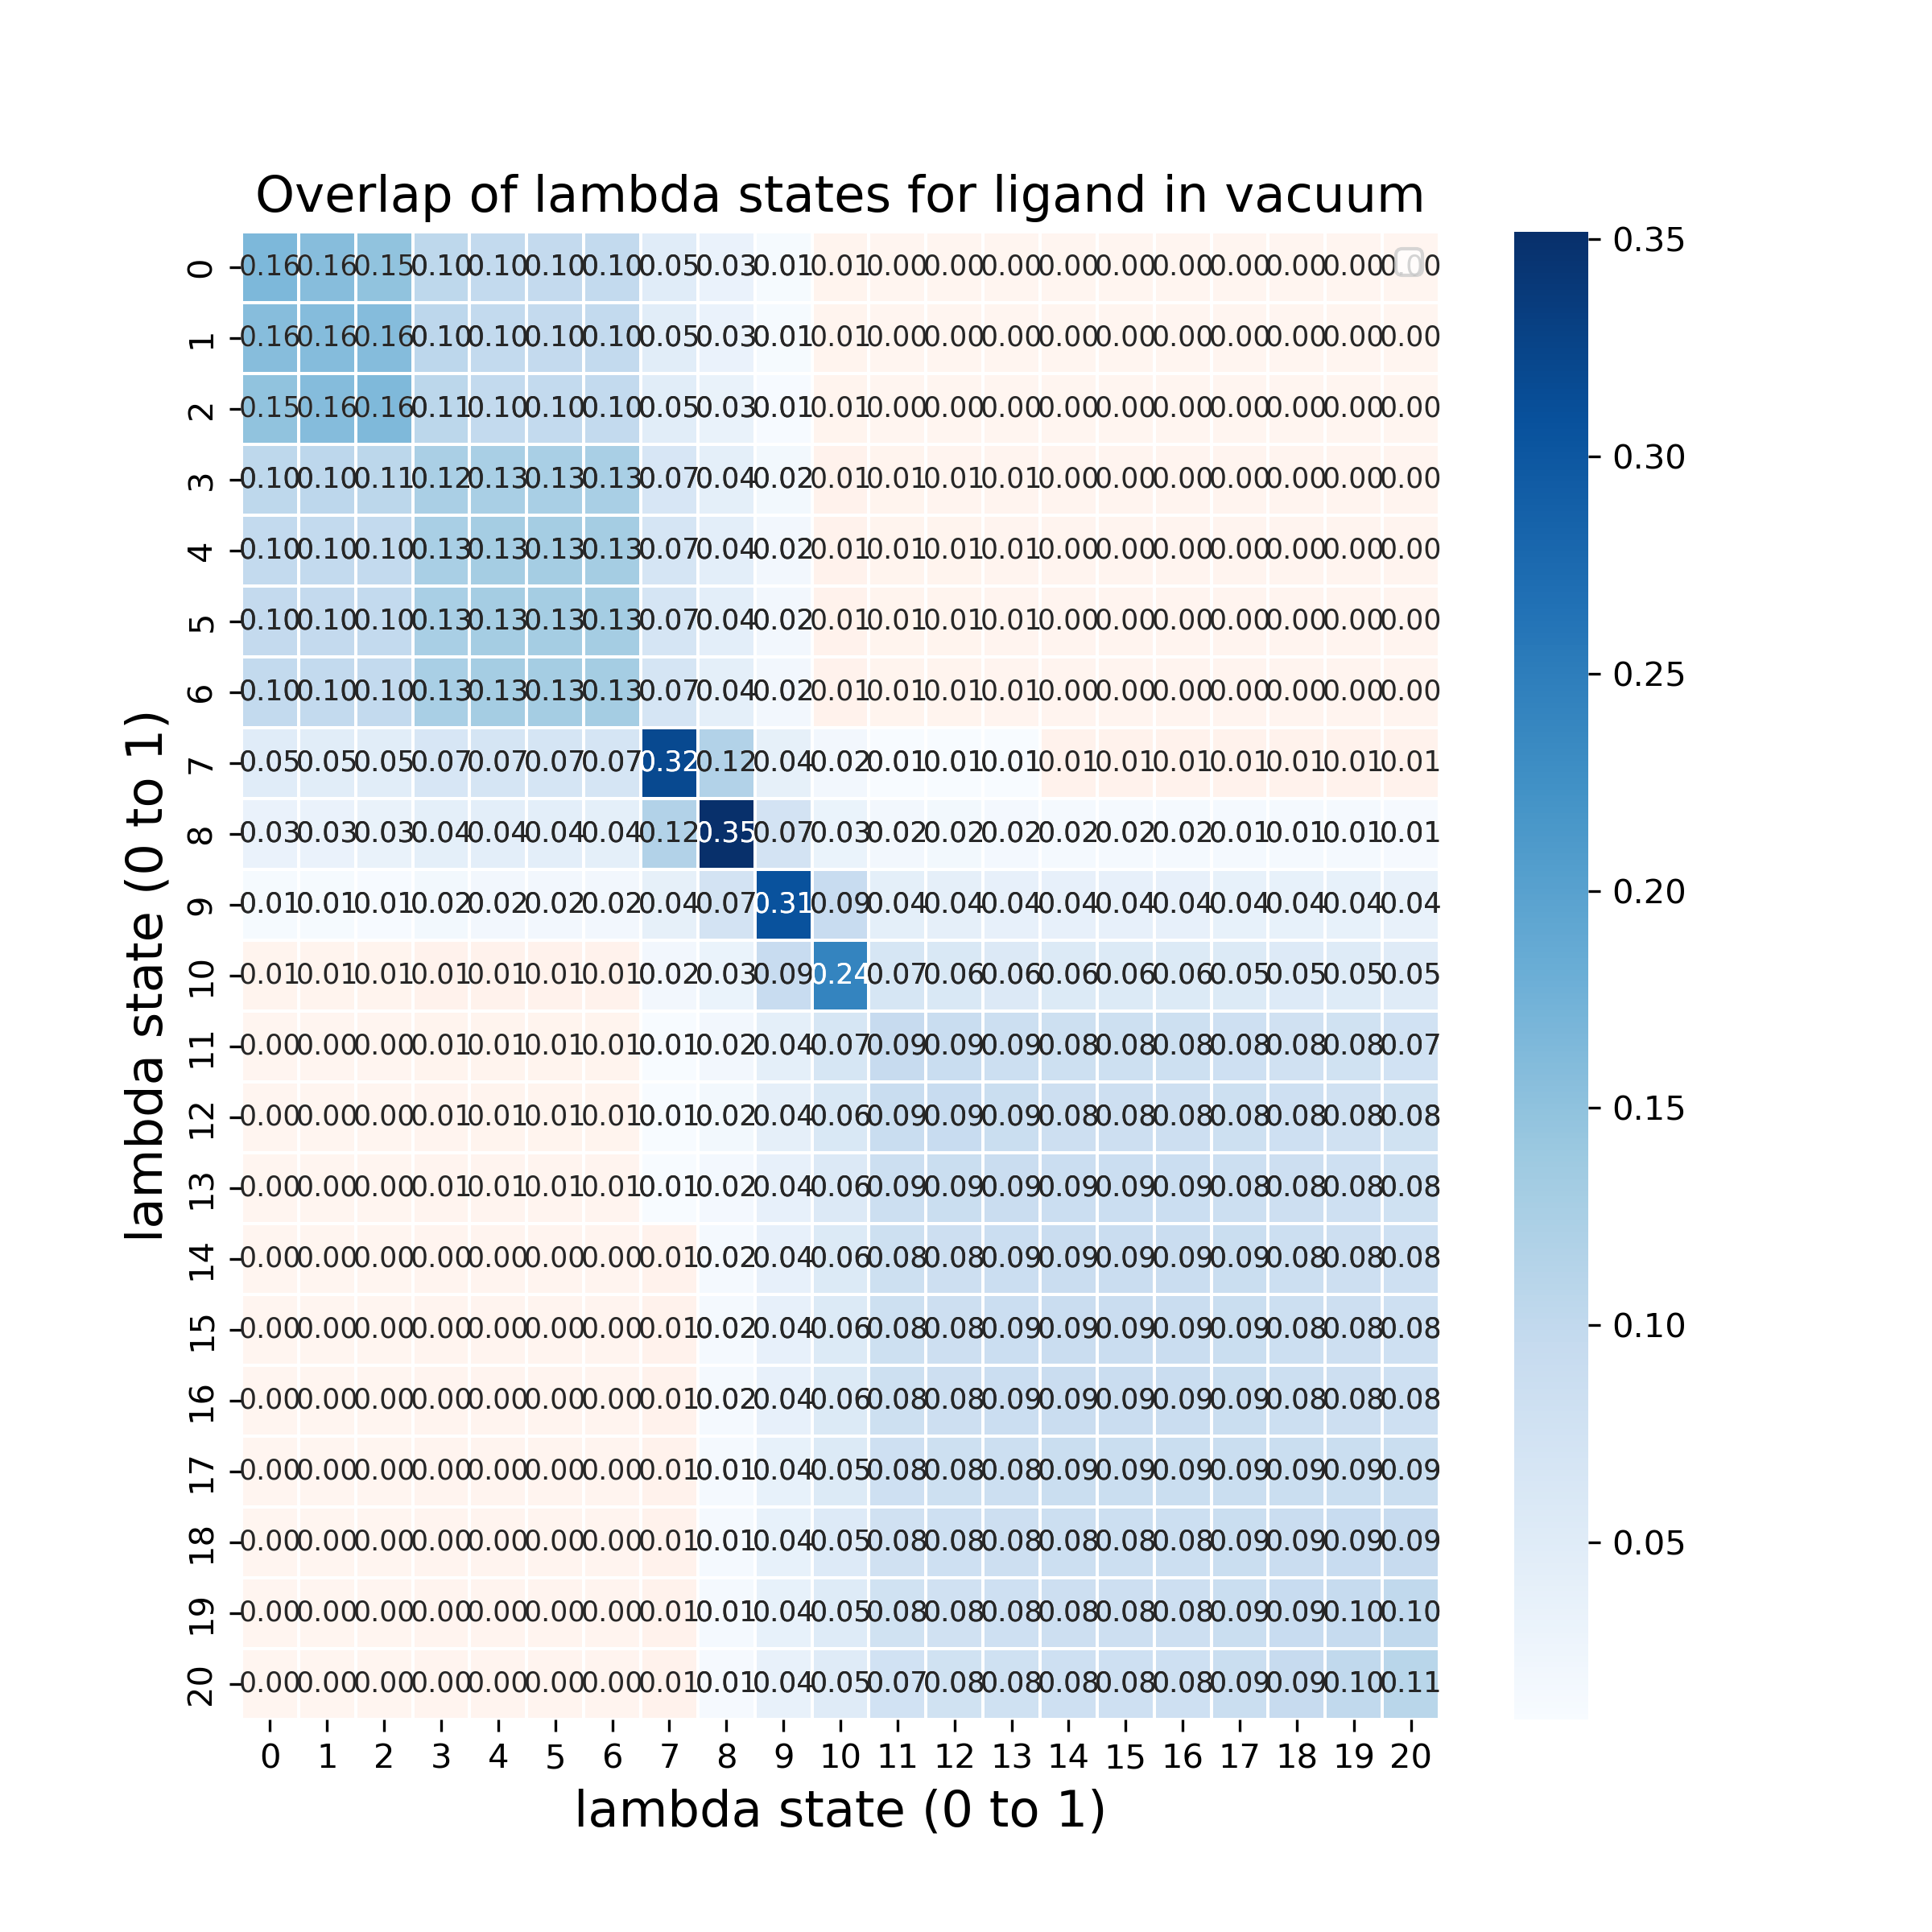
\includegraphics[width=0.4\textwidth]{overlap_vacuum_naphthol_old}%
		\label{fig:v_naphthol_old}%
	}\hfil
	\subfigure[naphthol/vacuum new]{%
		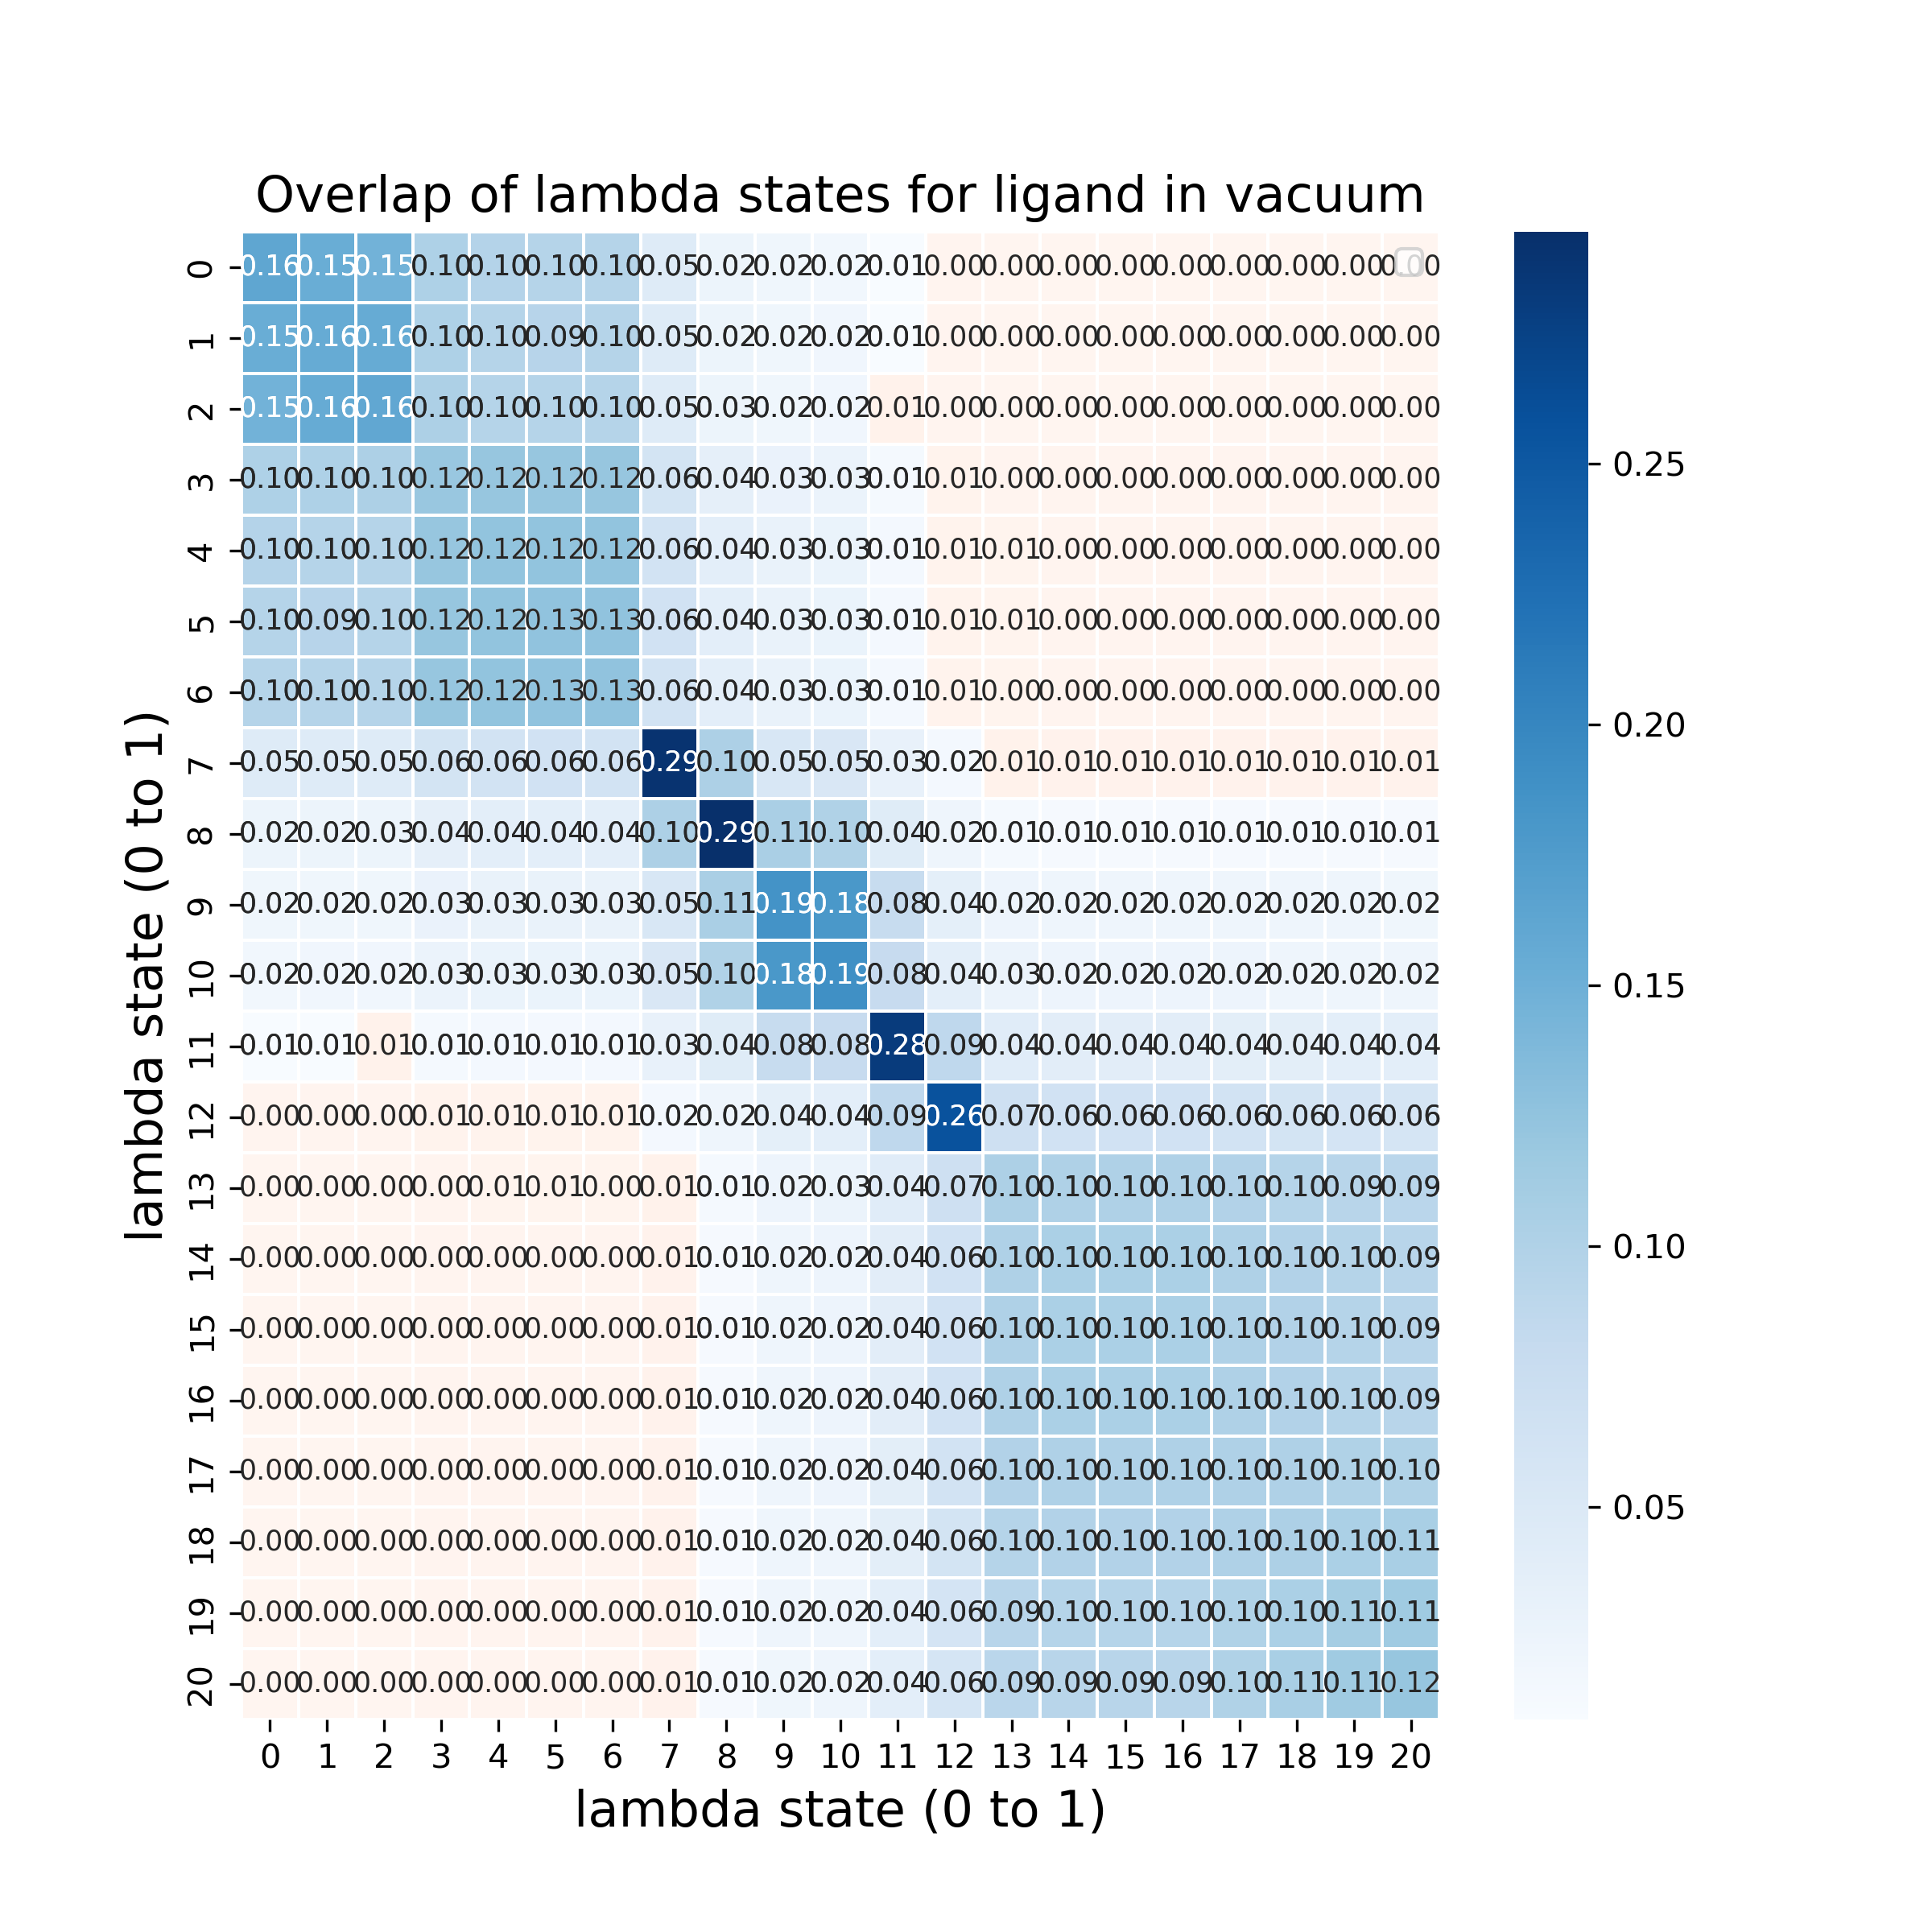
\includegraphics[width=0.4\textwidth]{overlap_vacuum_naphthol_new}%
		\label{fig:v_naphthol_new}%
	}
	
	\subfigure[naphthol/waterbox old]{%
		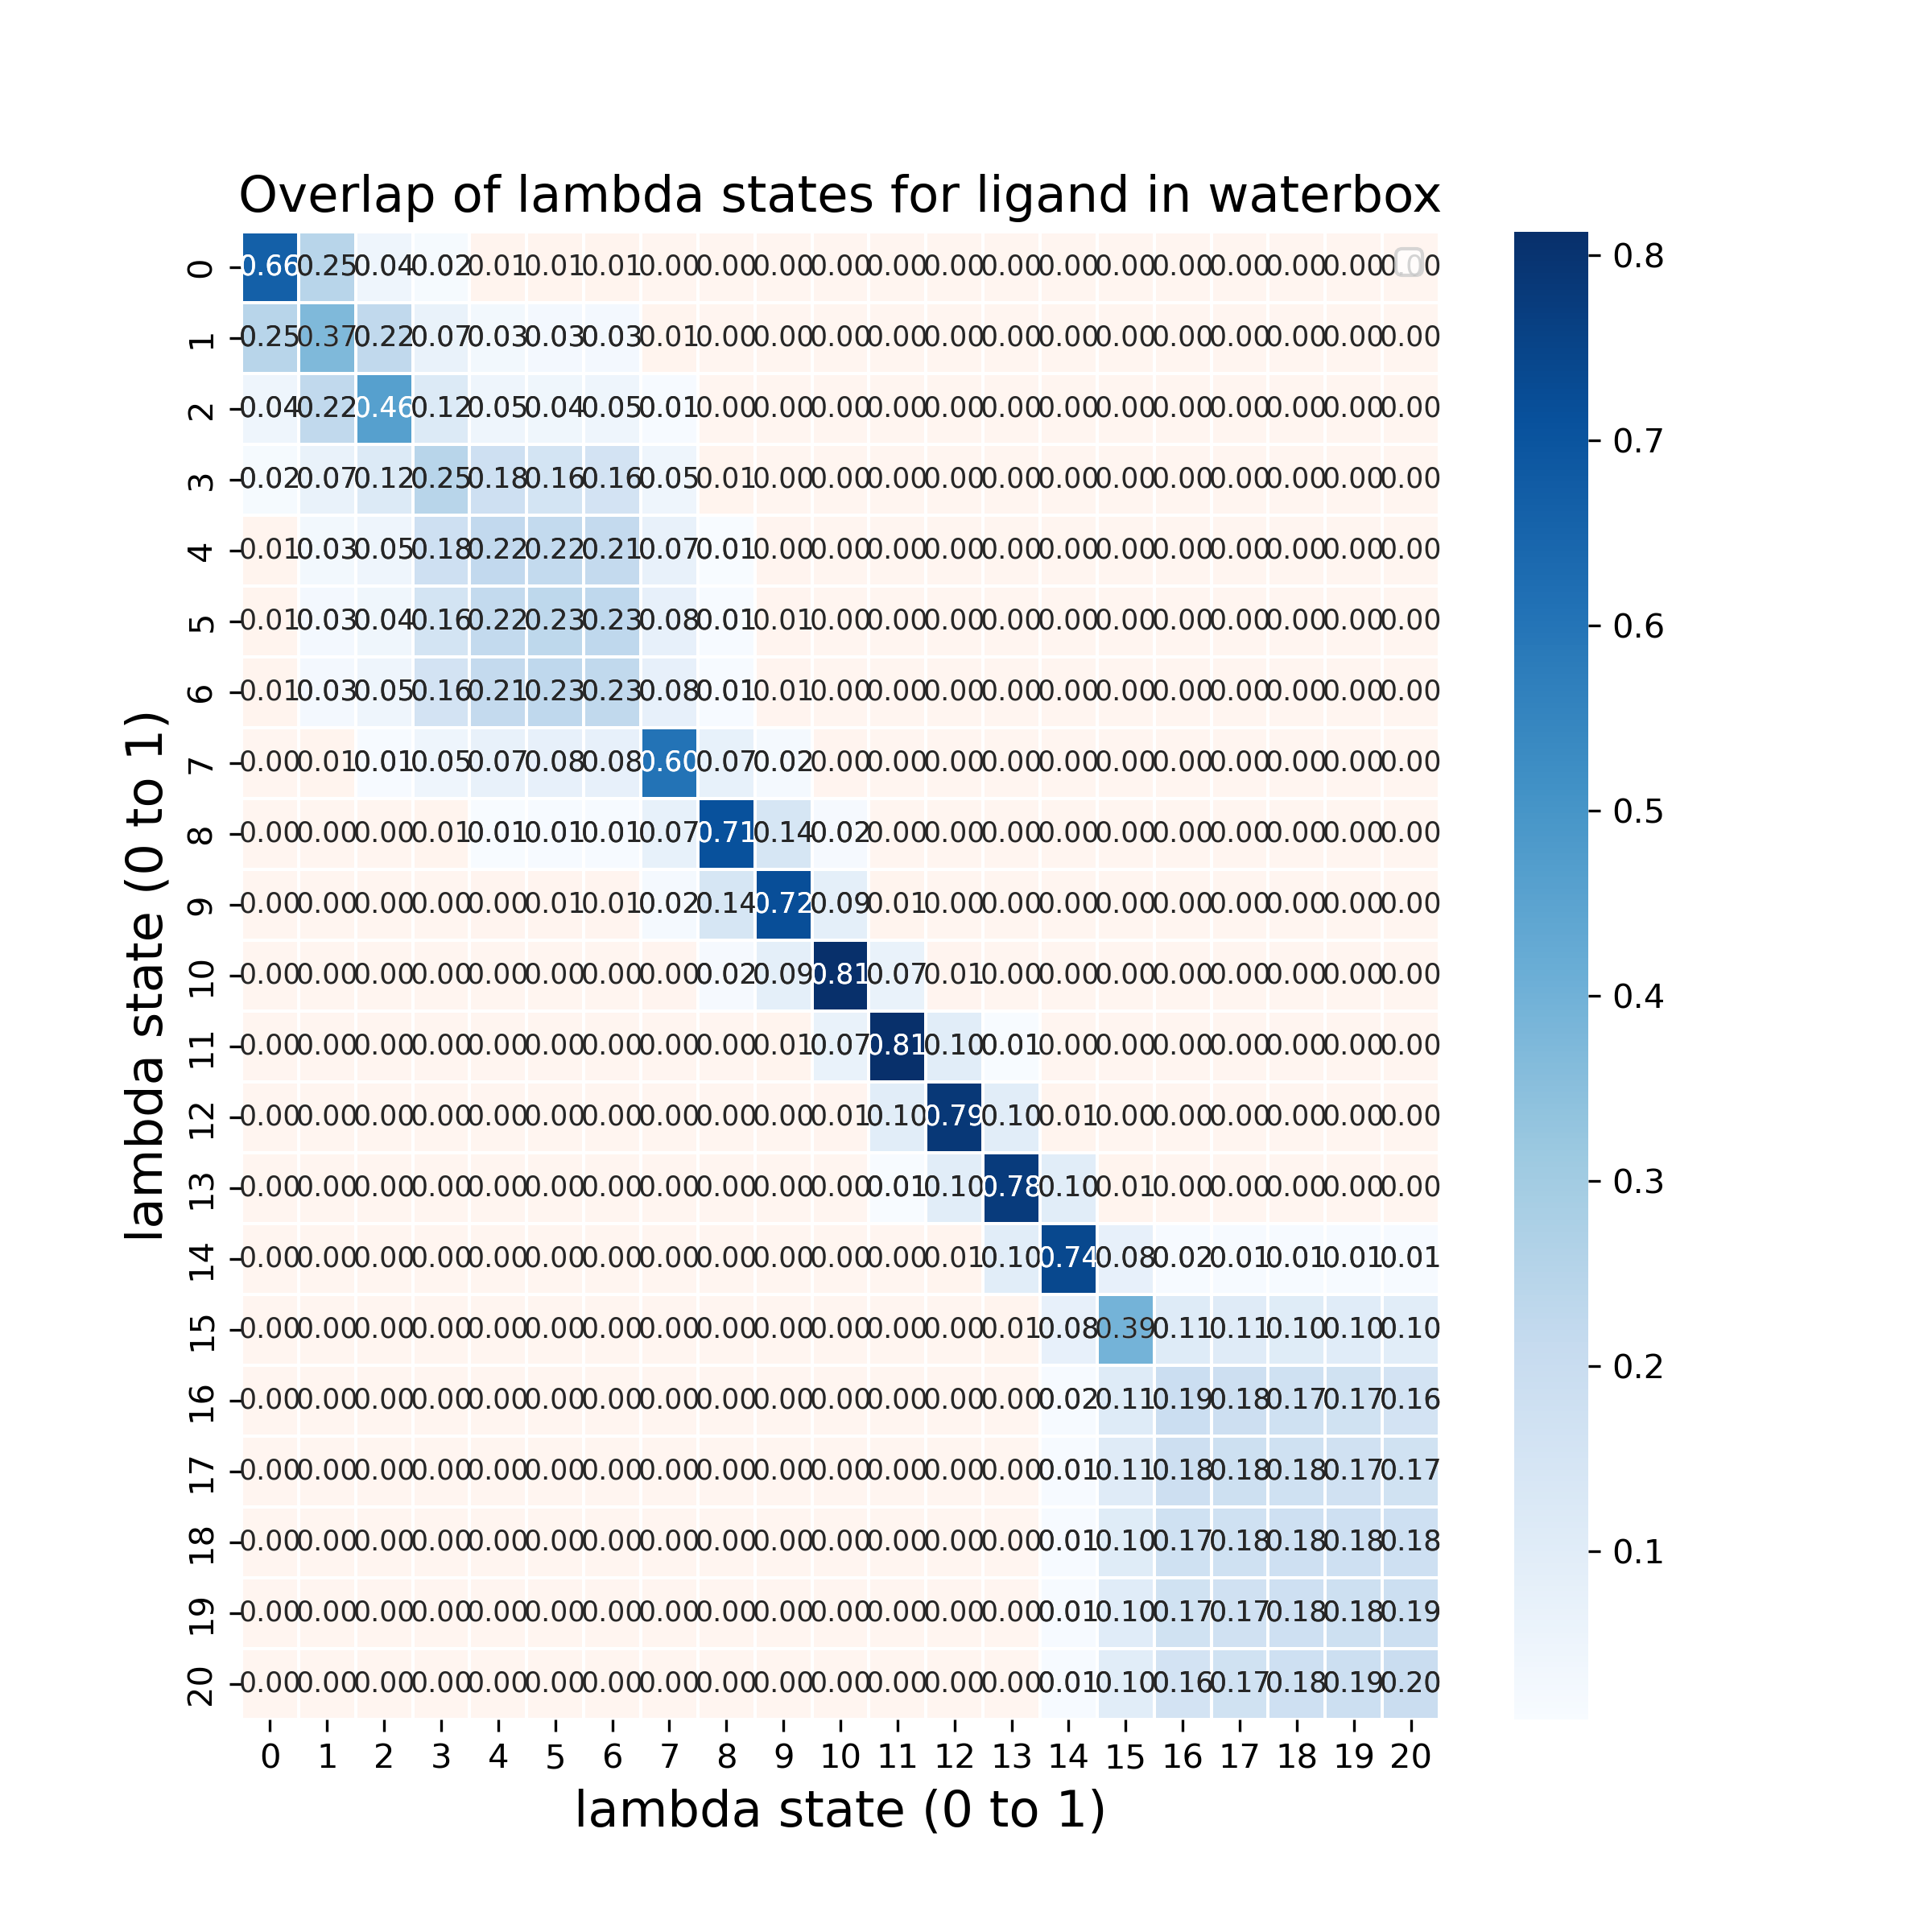
\includegraphics[width=0.4\textwidth]{overlap_waterbox_naphthol_old}%
		\label{fig:w_naphthol_old}%
	}\hfil
	\subfigure[naphthol/waterbox new]{%
		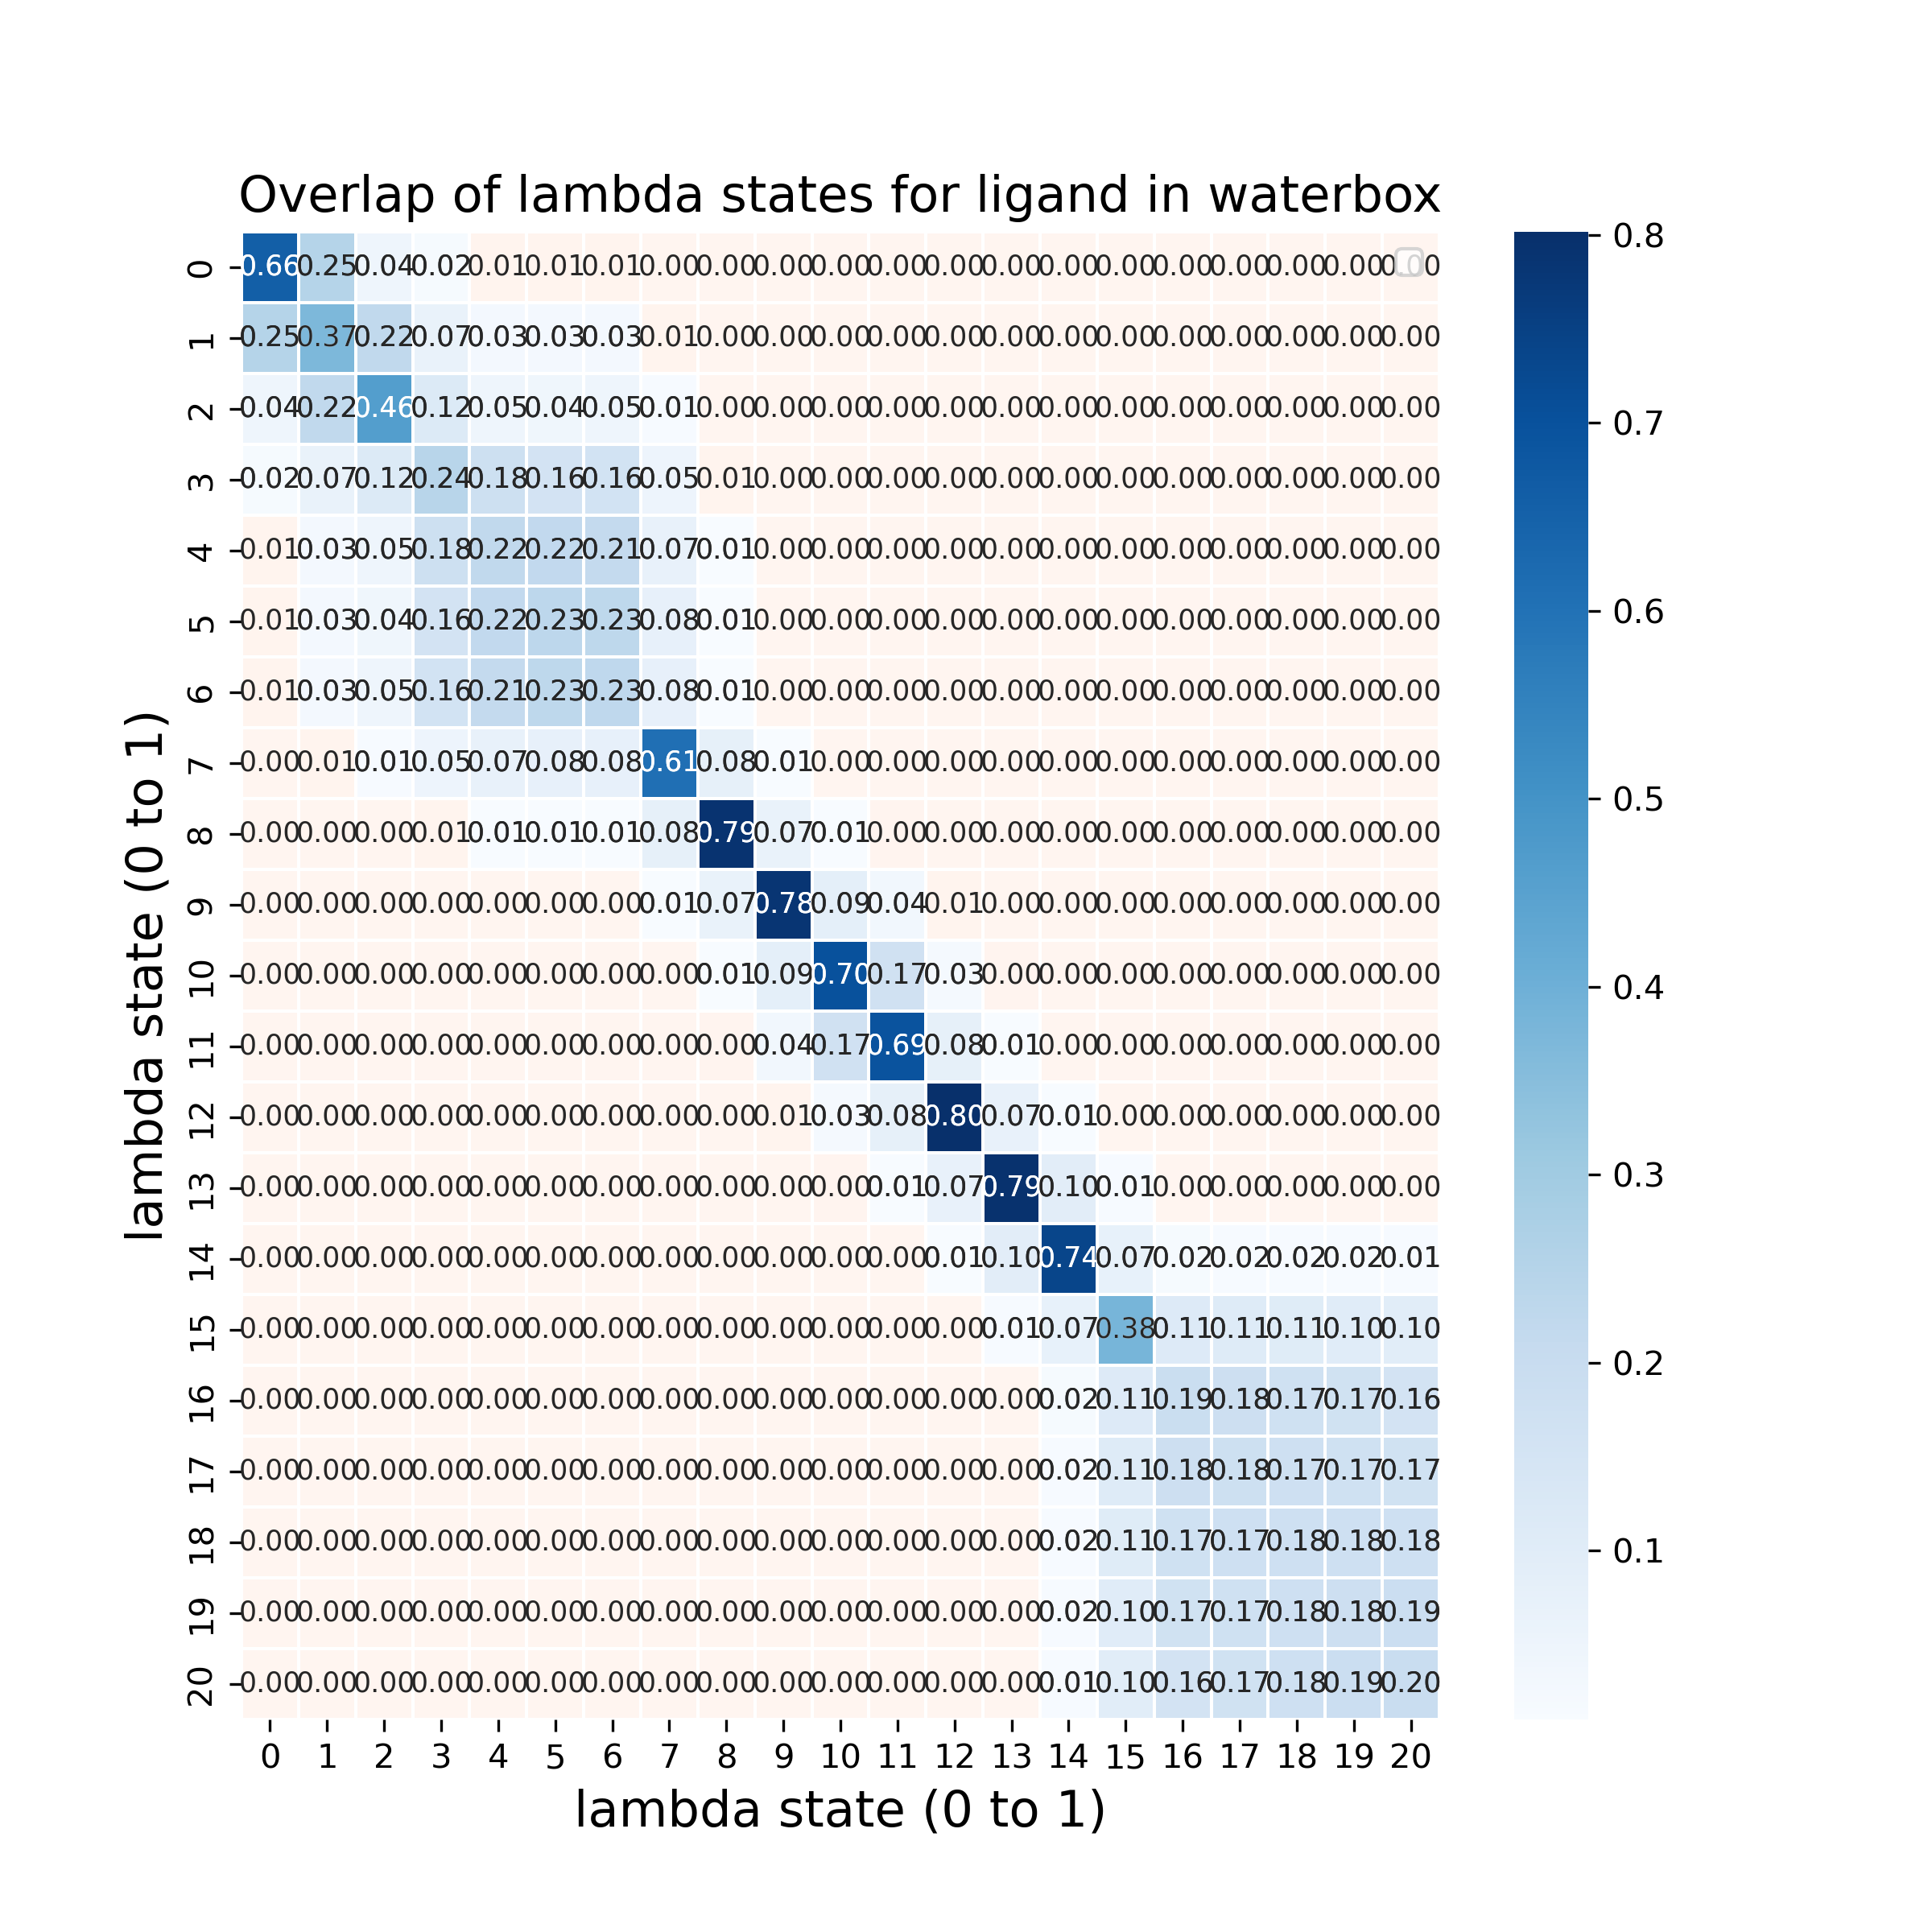
\includegraphics[width=0.4\textwidth]{overlap_waterbox_naphthol_new}%
		\label{fig:w_napthol_new}%
	}
	
	\caption{Overlap plots for naphthol: upper row: vacuum, lower row: waterbox; left: old mutation algorithm, right: new mutation algorithm}
\end{figure}

\begin{figure}[h] 
	\centering
	\subfigure[naphthol/vacuum old]{%
		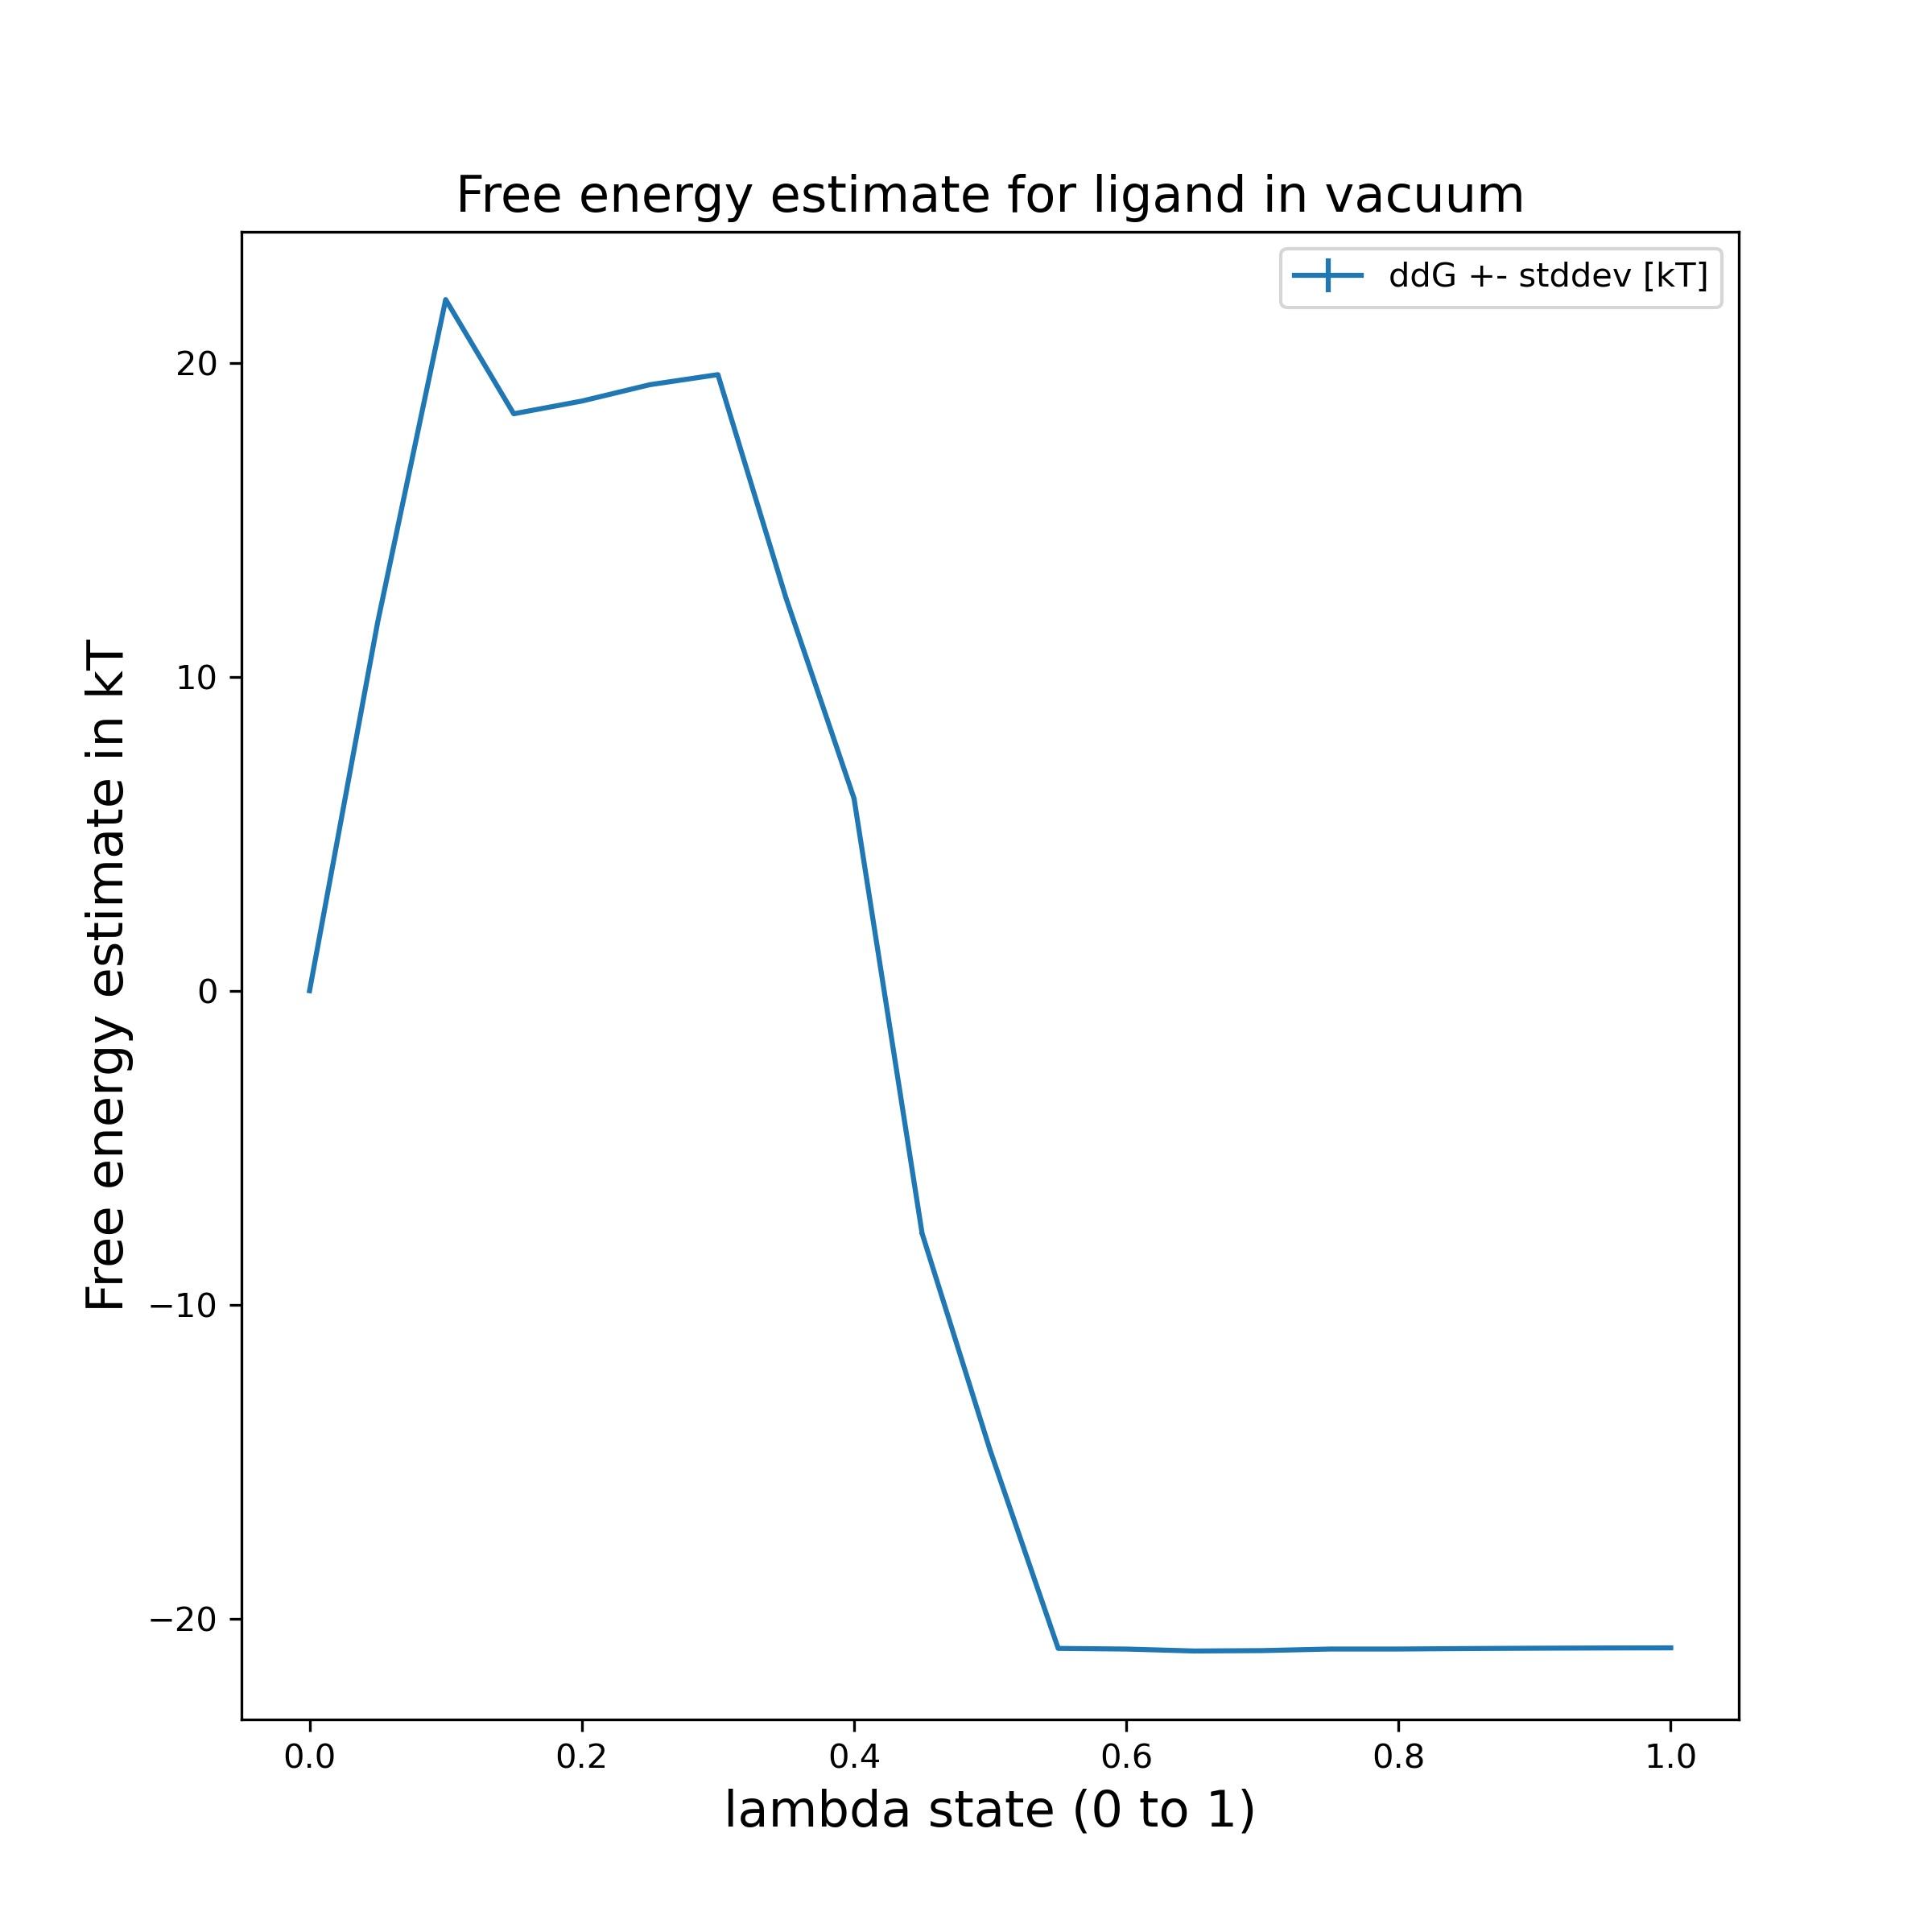
\includegraphics[width=0.4\textwidth]{states_vacuum_naphthol_old}%
		\label{fig:v_naphthol_oldstates}%
	}\hfil
	\subfigure[naphthol/vacuum new]{%
		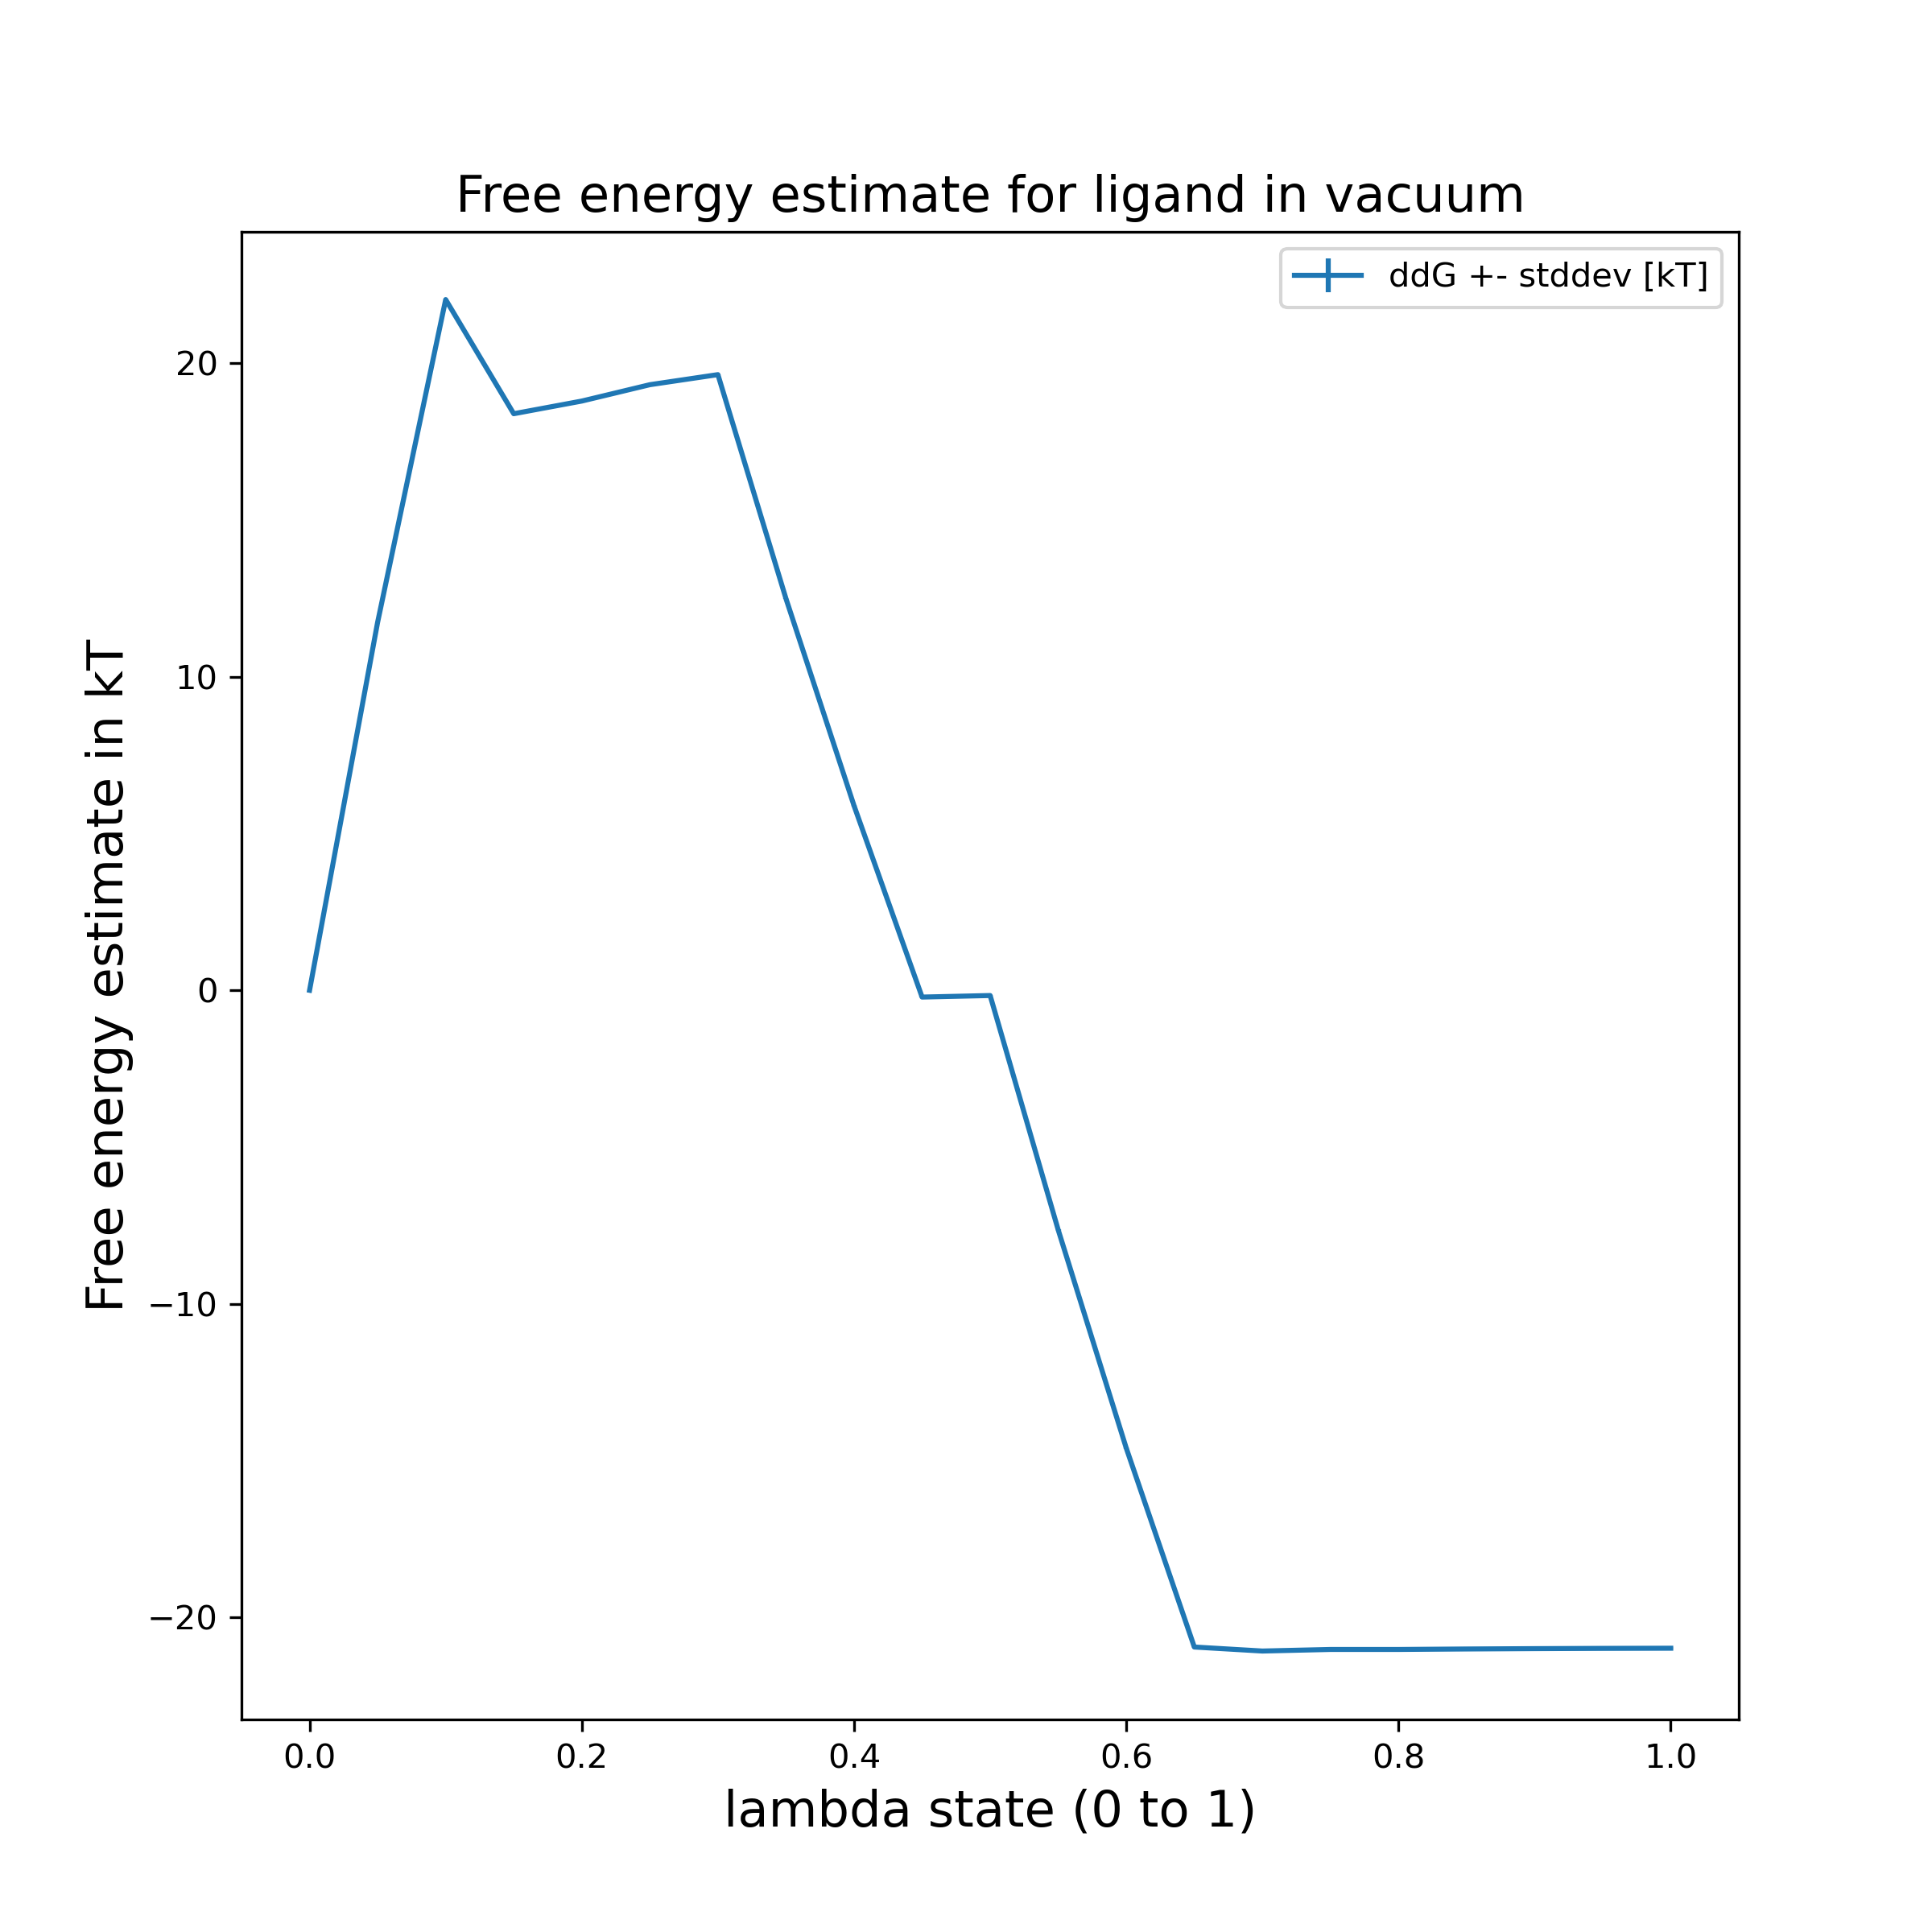
\includegraphics[width=0.4\textwidth]{states_vacuum_naphthol_new}%
		\label{fig:v_naphthol_newstates}%
	}
	\subfigure[naphthol/waterbox old]{%
		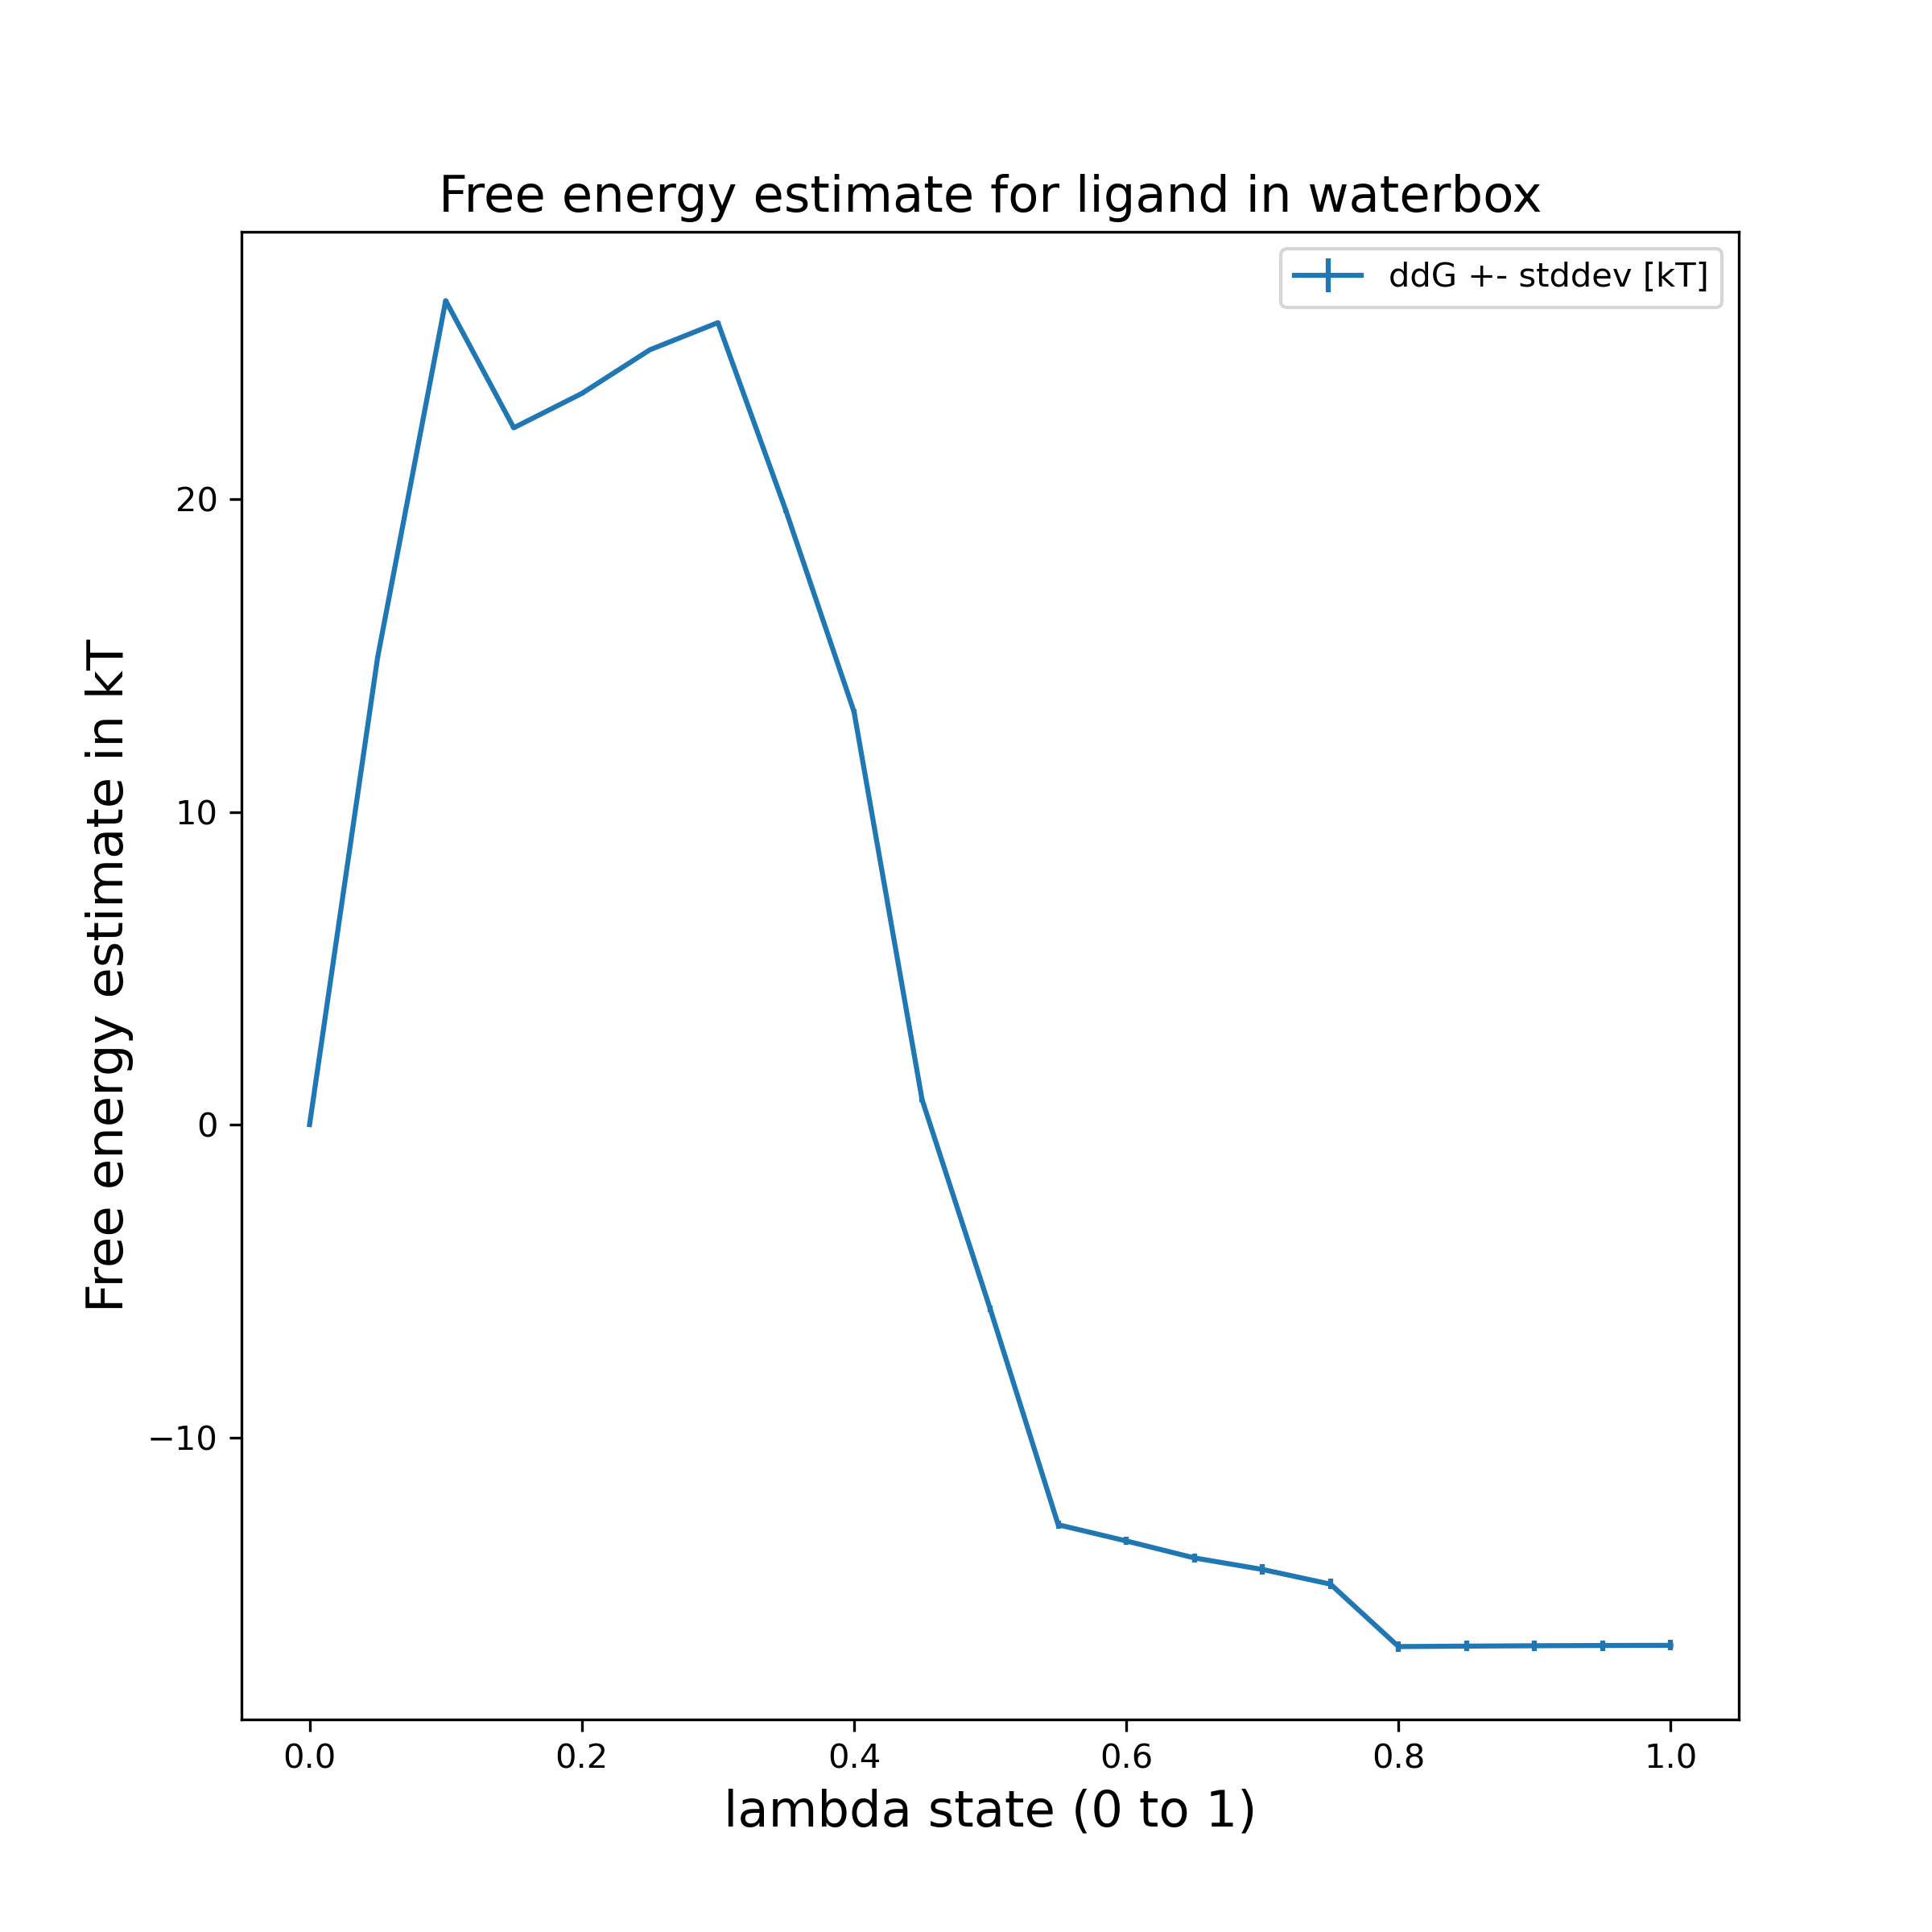
\includegraphics[width=0.43\textwidth]{states_waterbox_naphthol_old}%
		\label{fig:w_naphthol_oldstates}%
	}\hfil
	\subfigure[naphthol/waterbox new]{%
		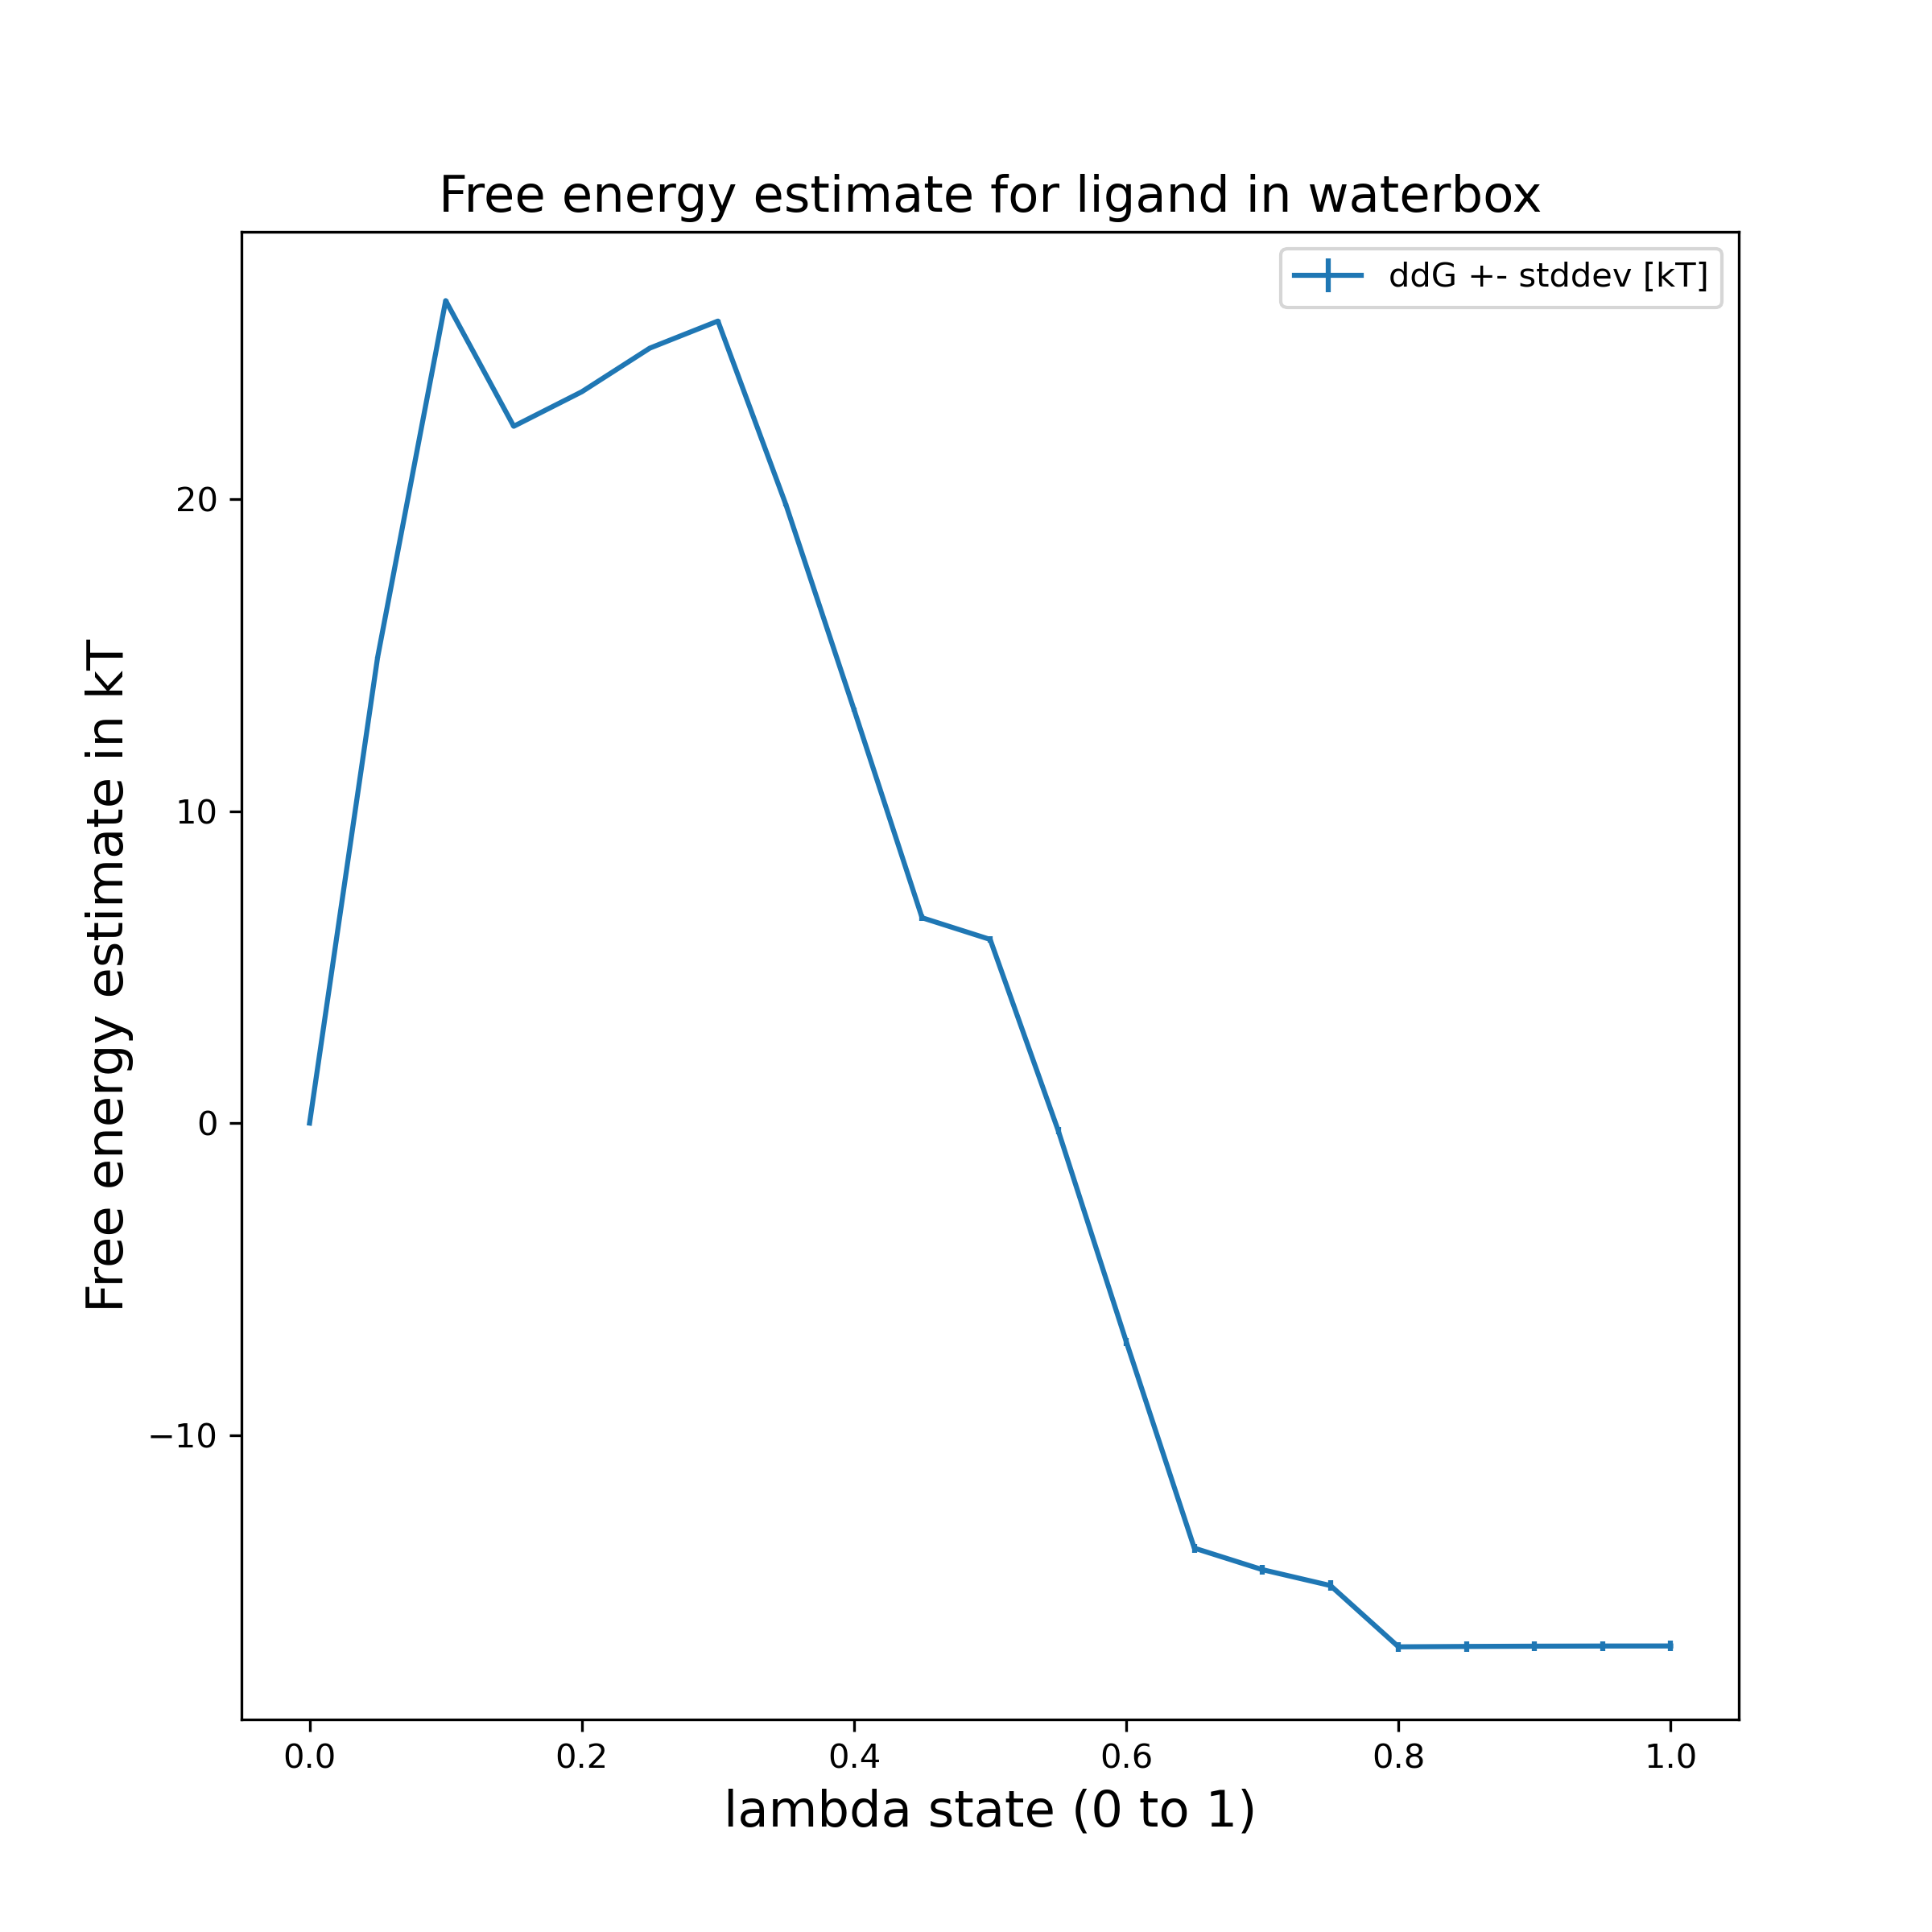
\includegraphics[width=0.4\textwidth]{states_waterbox_naphthol_new}%
		\label{fig:w_napthol_newstates}%
	}
	
	\caption{Free energy states at different lambda states for naphthol: upper row: vacuum, lower row: waterbox; left: old mutation algorithm, right: new mutation algorithm}
\end{figure}

\begin{figure}[h]
	\centering
	\subfigure[toluene/vacuum old]{%
		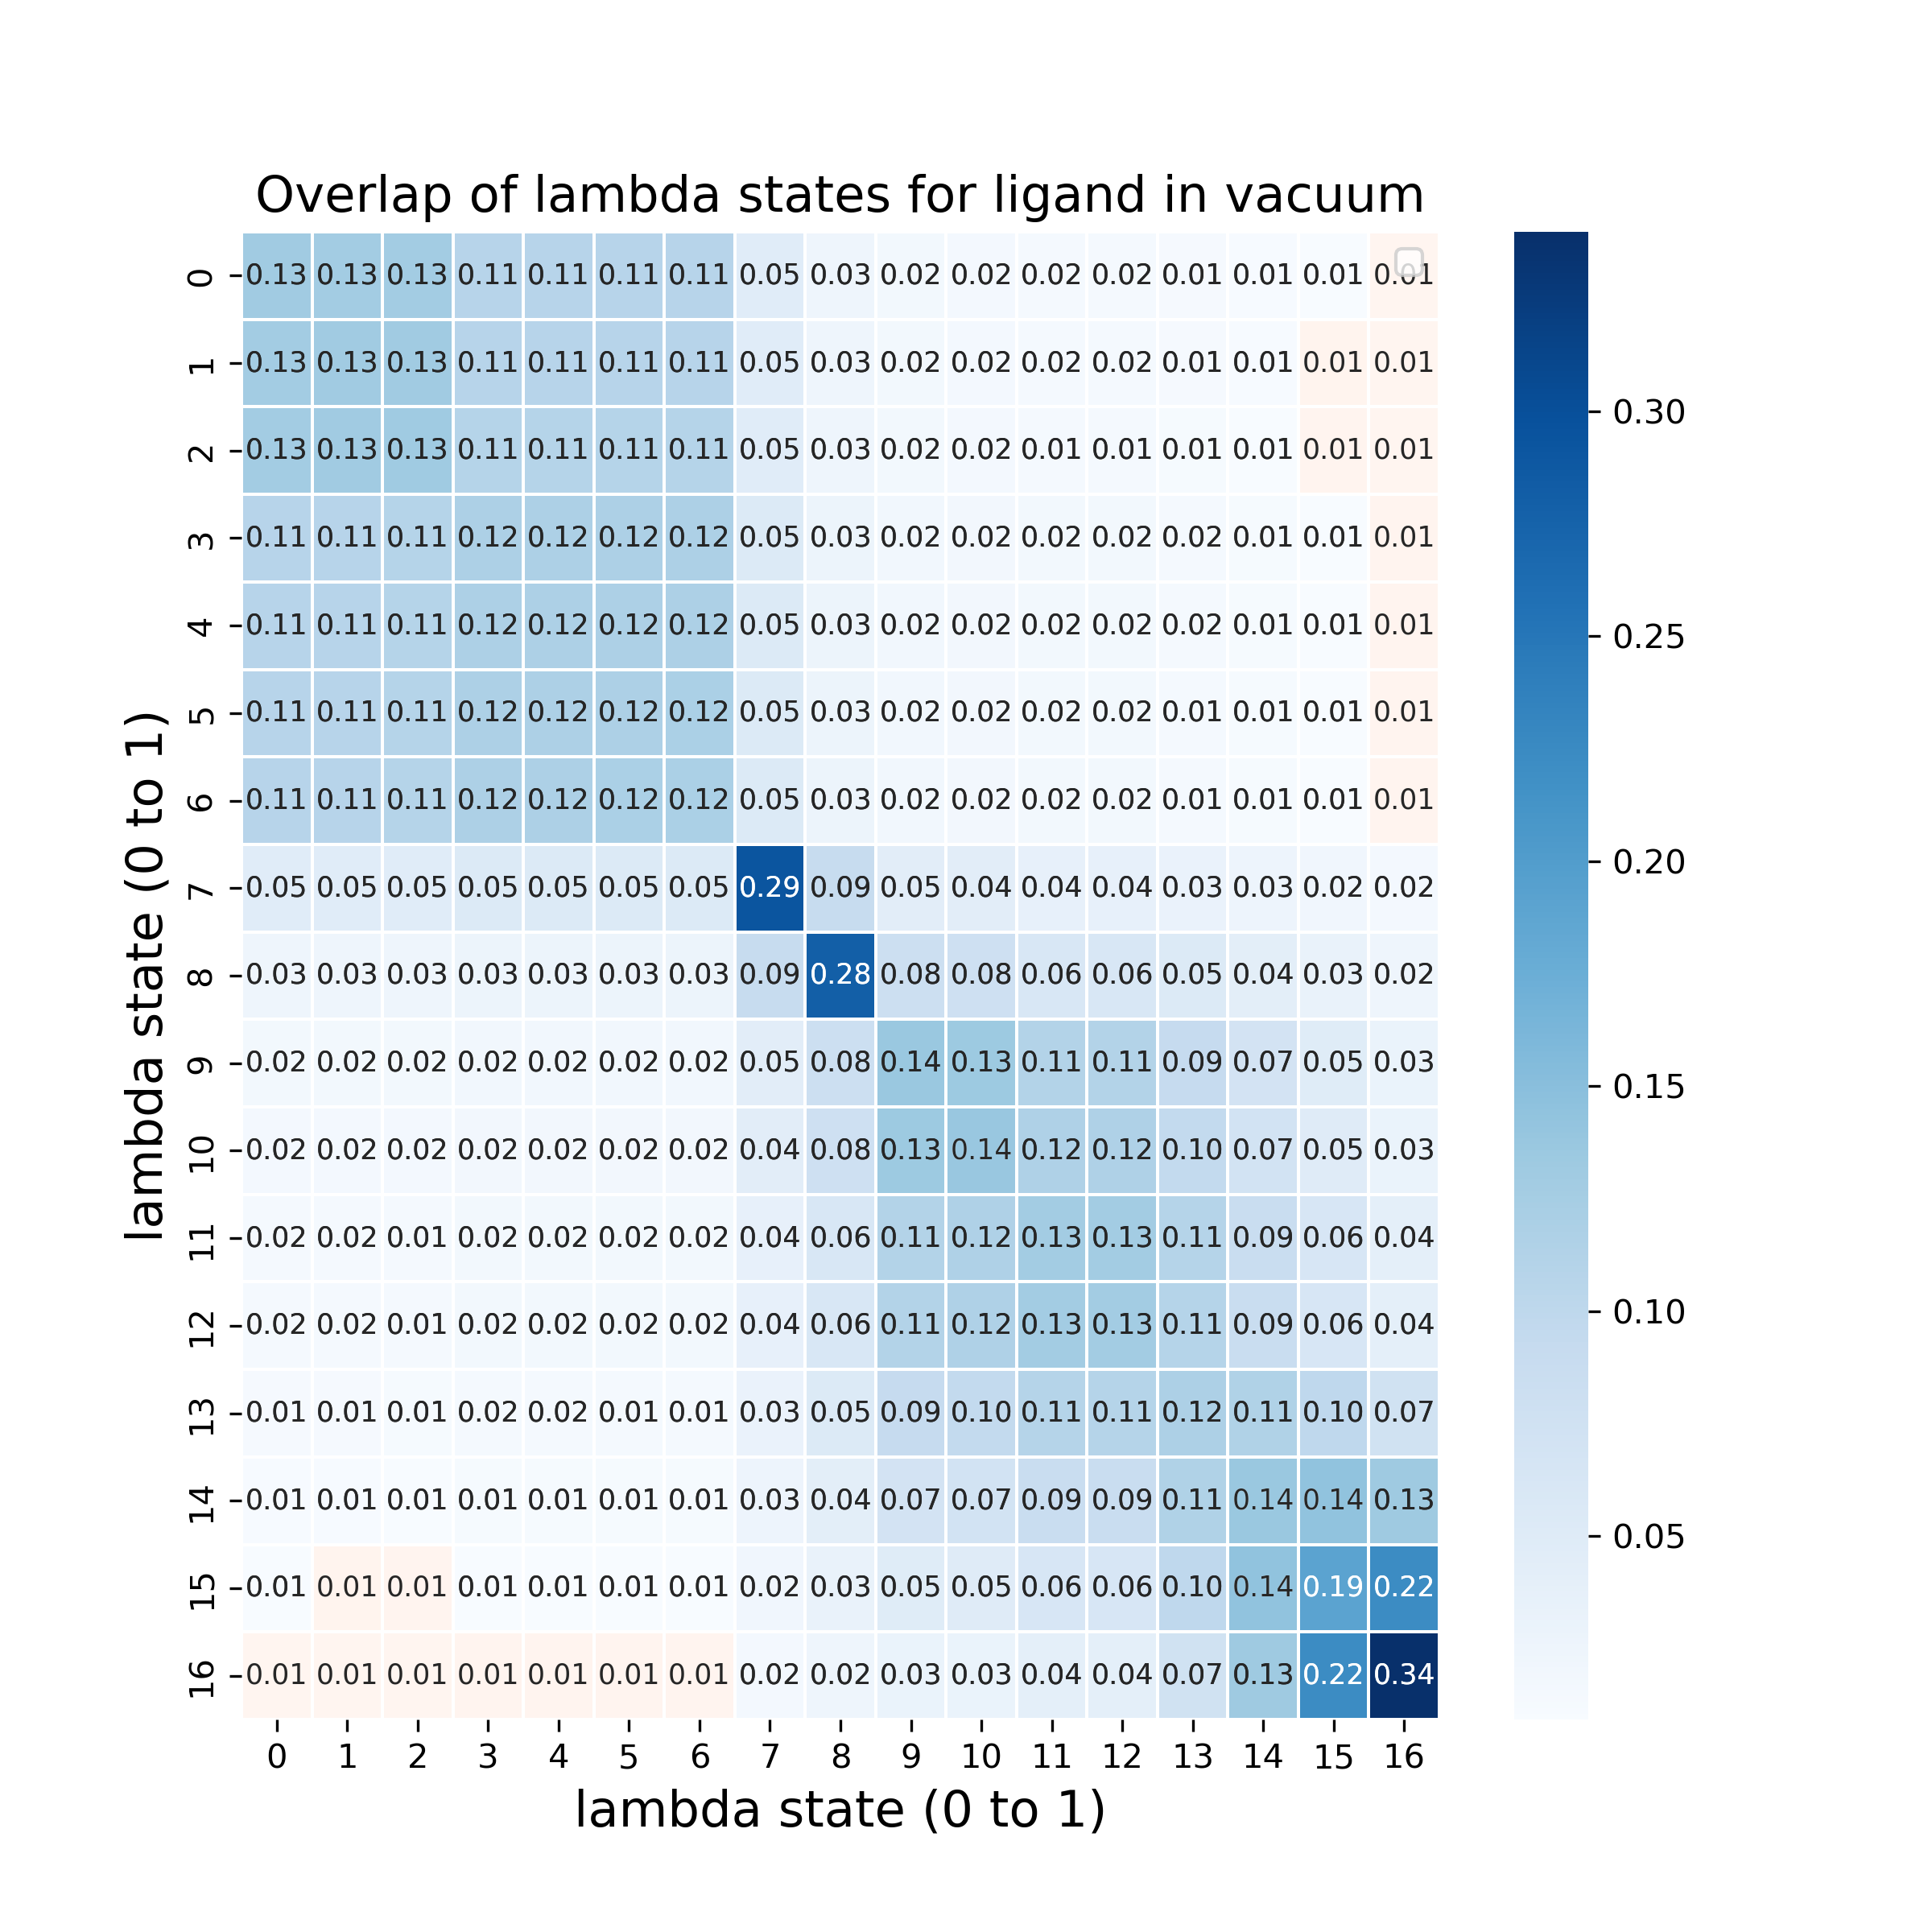
\includegraphics[width=0.4\textwidth]{overlap_vacuum_toluene_old}%
		\label{fig:v_toluene_old}%
	}\hfil
	\subfigure[toluene/vacuum new]{%
		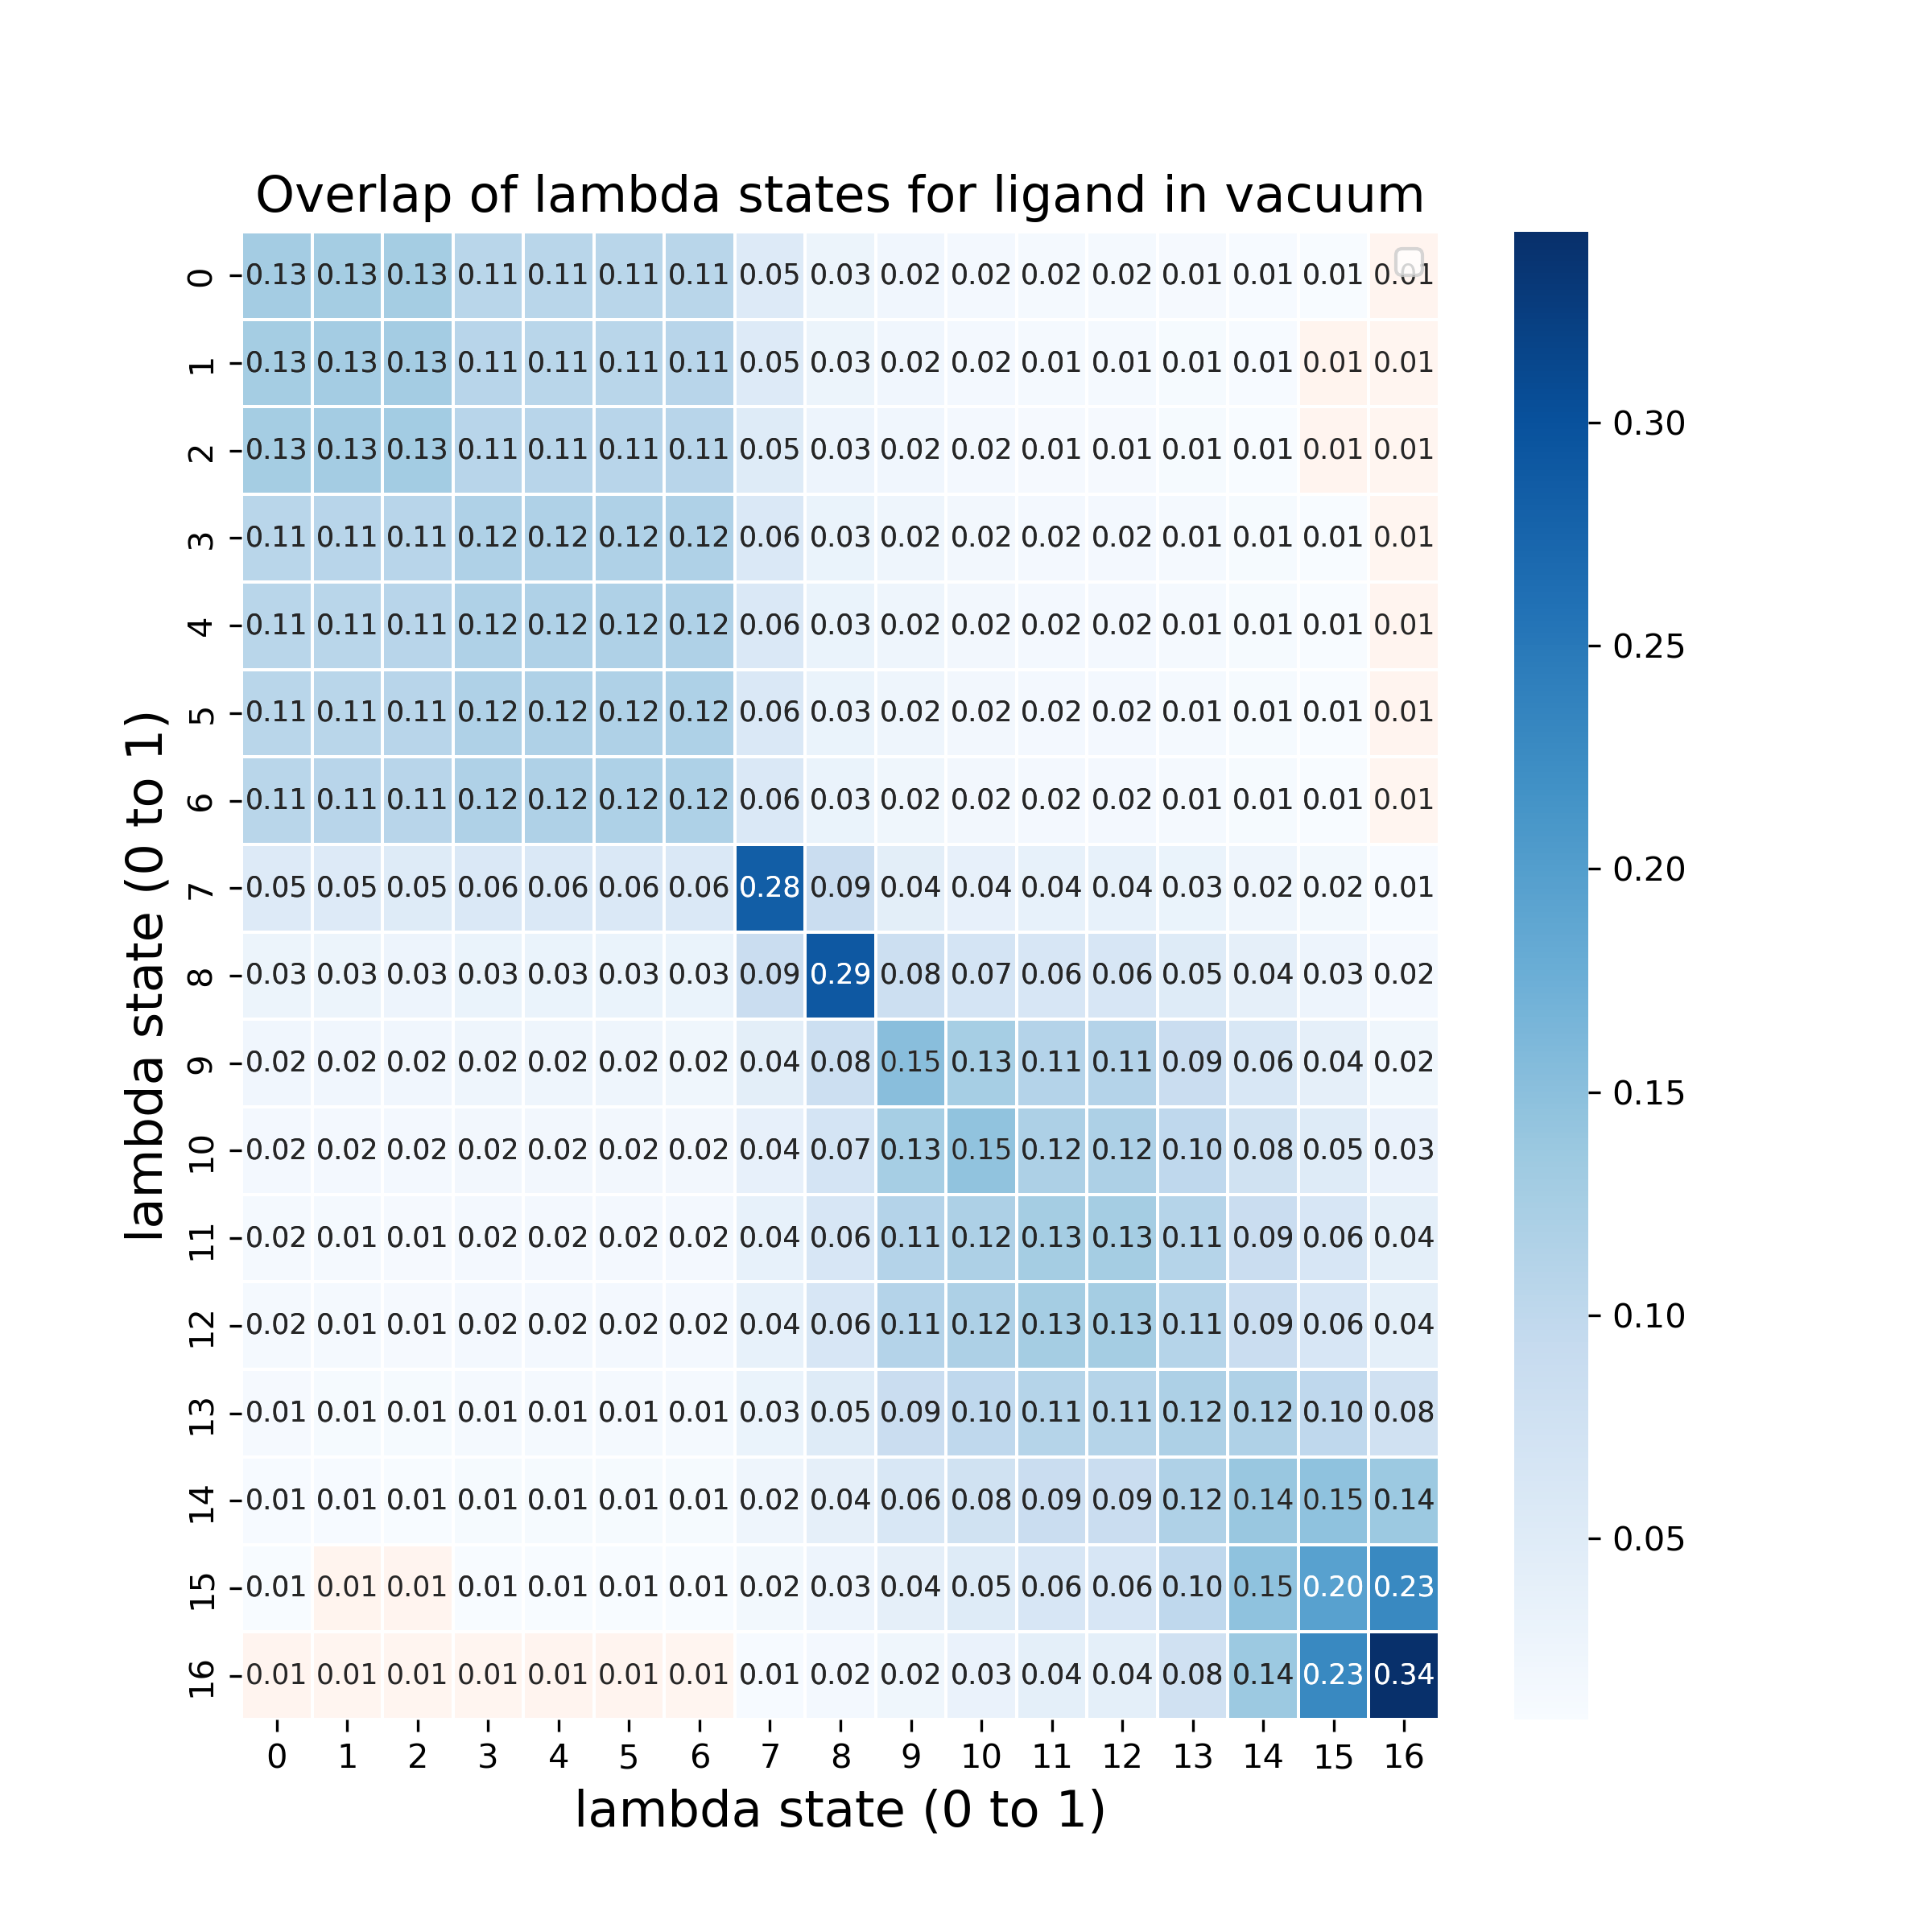
\includegraphics[width=0.4\textwidth]{overlap_vacuum_toluene_new}%
		\label{fig:v_toluene_new}%
	}
	
	\subfigure[toluene/waterbox old]{%
		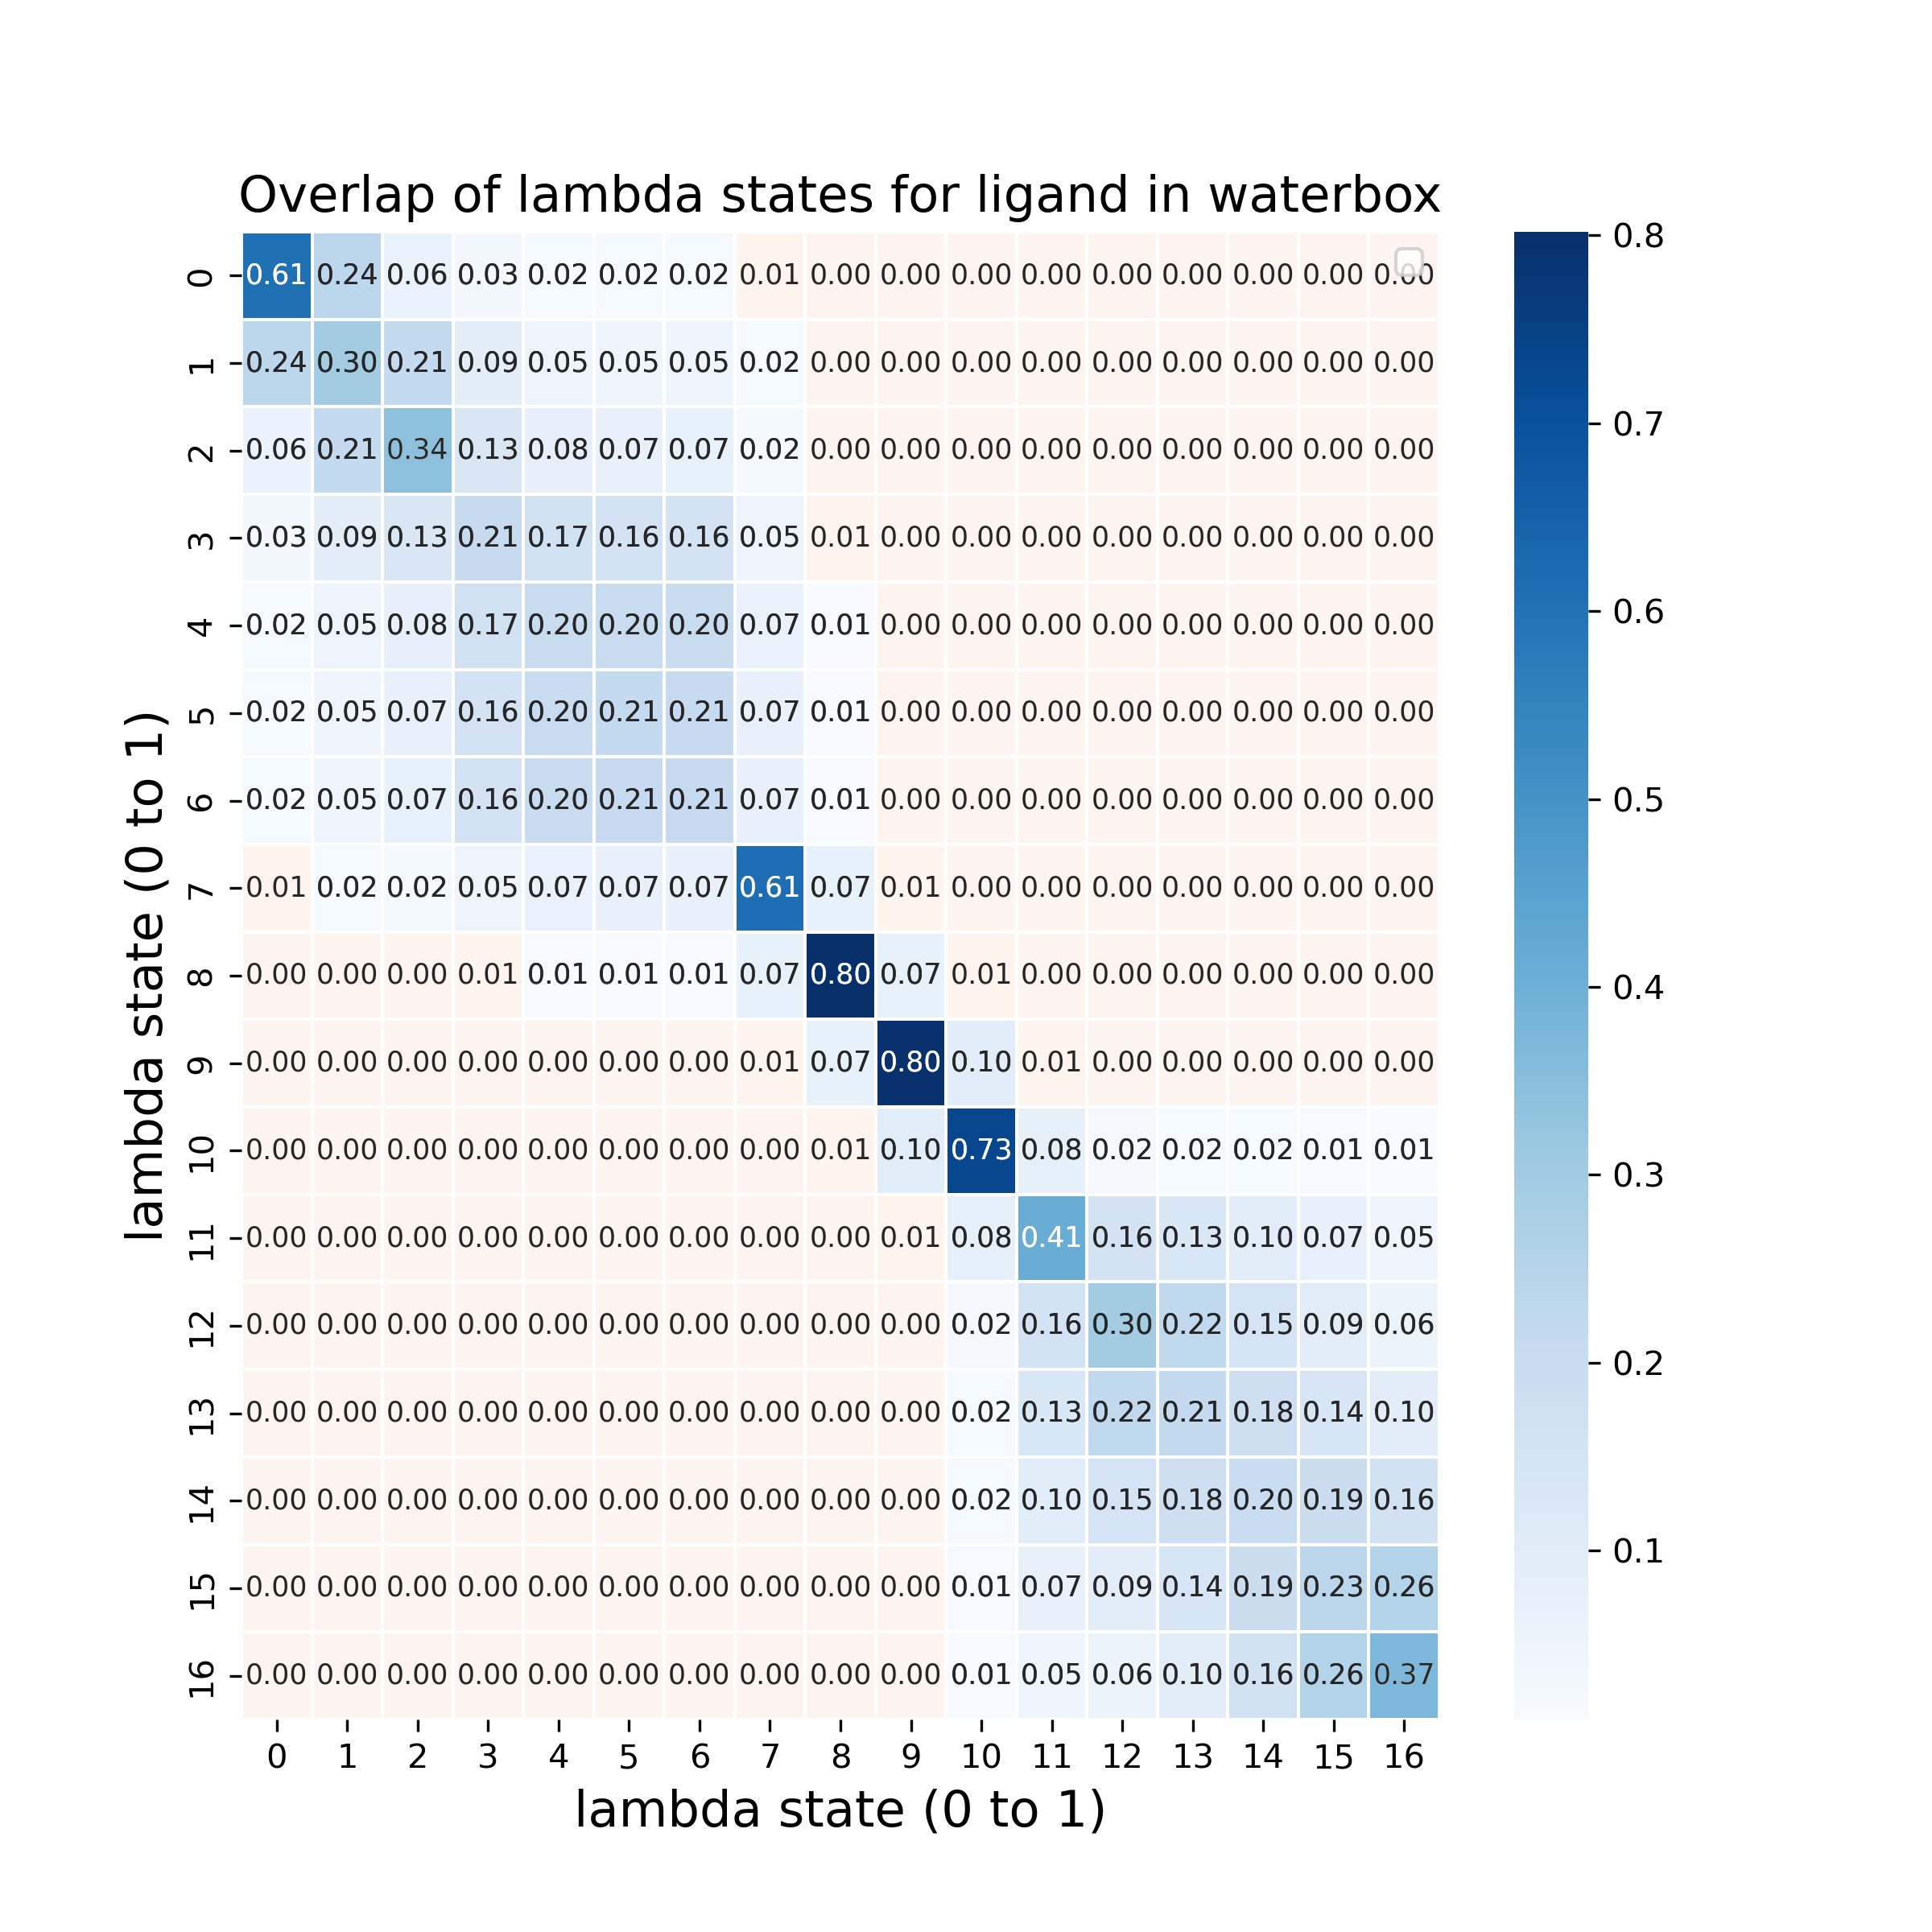
\includegraphics[width=0.4\textwidth]{overlap_waterbox_toluene_old}%
		\label{fig:w_toluene_old}%
	}\hfil
	\subfigure[toluene/waterbox new]{%
		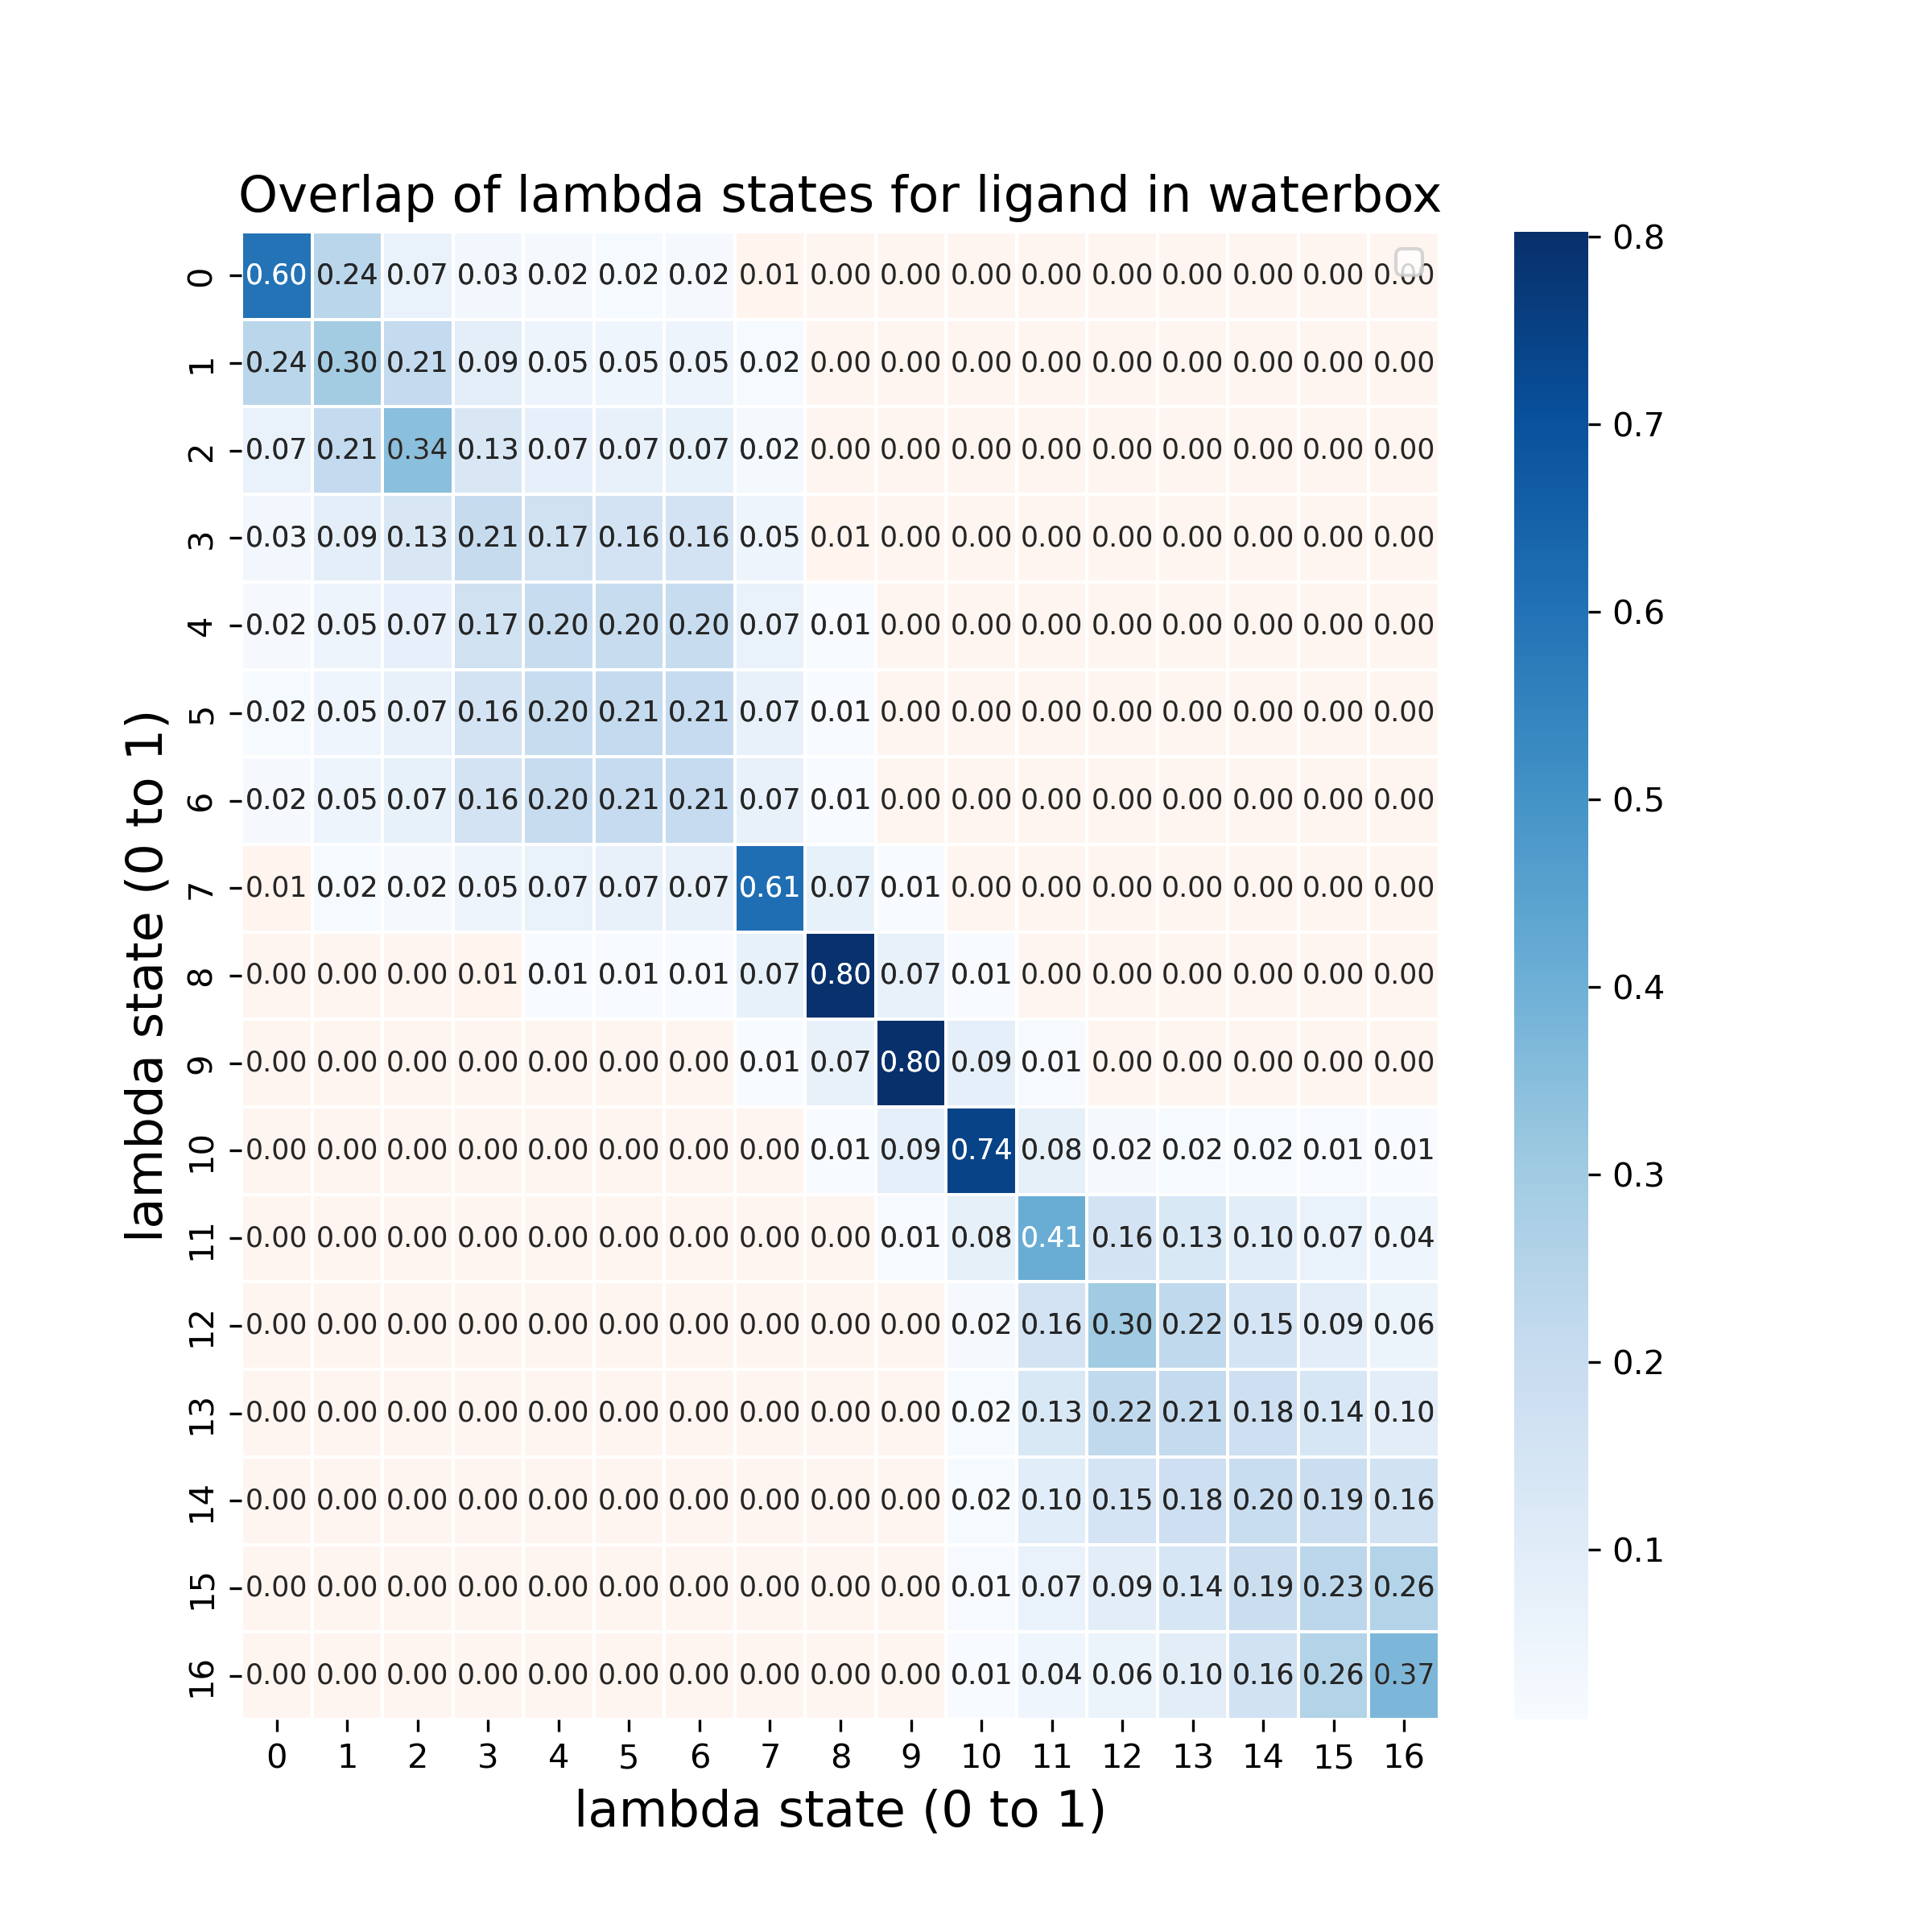
\includegraphics[width=0.4\textwidth]{overlap_waterbox_toluene_new}%
		\label{fig:w_toluene_new}%
	}
	
	\caption{Overlap plots for toluene: upper row: vacuum, lower row: waterbox; left: old mutation algorithm, right: new mutation algorithm}
\end{figure}

